%%%%%%%%%%%%%%%%%%%%%%%%%%%%%%%%%%%%%%%%%%%%%%%%%
% Spacedrive V2 Whitepaper Template
% Version 2.0 - Incorporating Advanced Concepts
%%%%%%%%%%%%%%%%%%%%%%%%%%%%%%%%%%%%%%%%%%%%%%%%%
\documentclass[sigconf]{acmart}

% Code formatting packages
\usepackage{listings}
\usepackage{xcolor}
\usepackage{enumitem}
\usepackage{booktabs}
\usepackage{tikz}
\usetikzlibrary{shapes.geometric, arrows.meta, positioning, shadows, patterns, fit, backgrounds}
\usepackage{pgfplots}
\pgfplotsset{compat=1.17}

% Define colors for code highlighting
\definecolor{codegreen}{rgb}{0,0.6,0}
\definecolor{codegray}{rgb}{0.5,0.5,0.5}
\definecolor{codepurple}{rgb}{0.58,0,0.82}
\definecolor{backcolour}{rgb}{0.95,0.95,0.92}
\definecolor{keywordblue}{rgb}{0,0,0.8}

% Style for Rust code
\lstdefinestyle{ruststyle}{
 backgroundcolor=\color{backcolour},
 commentstyle=\color{codegreen},
 keywordstyle=\color{keywordblue},
 numberstyle=\tiny\color{codegray},
 stringstyle=\color{codepurple},
 basicstyle=\ttfamily\footnotesize,
 breakatwhitespace=false,
 breaklines=true,
 captionpos=b,
 keepspaces=true,
 numbers=left,
 numbersep=5pt,
 showspaces=false,
 showstringspaces=false,
 showtabs=false,
 tabsize=2,
 frame=single,
 rulecolor=\color{black!30}
}

% Style for SQL
\lstdefinestyle{sqlstyle}{
 backgroundcolor=\color{backcolour},
 commentstyle=\color{codegreen},
 keywordstyle=\color{keywordblue},
 stringstyle=\color{codepurple},
 basicstyle=\ttfamily\footnotesize,
 numbers=left,
 numbersep=5pt,
 frame=single,
 rulecolor=\color{black!30},
 breaklines=true
}

% Style for shell/config
\lstdefinestyle{shellstyle}{
 backgroundcolor=\color{backcolour},
 commentstyle=\color{codegreen},
 basicstyle=\ttfamily\footnotesize,
 numbers=left,
 numbersep=5pt,
 frame=single,
 rulecolor=\color{black!30},
 breaklines=true
}

% Define Rust language for listings
\lstdefinelanguage{Rust}{
 keywords={
  as, async, await, break, const, continue, crate, dyn, else, enum, extern, false, fn, for, if, impl, in, let, loop, match, mod, move, mut, pub, ref, return, self, Self, static, struct, super, trait, true, type, unsafe, use, where, while
 },
 morecomment=[l]{//},
 morecomment=[s]{/*}{*/},
 morestring=[b]",
 morestring=[b]',
 sensitive=true,
}

\lstset{style=ruststyle} % Set default style

% --- METADATA ---
\acmConference[Spacedrive '25]{Spacedrive Whitepaper}{July 26, 2025}{Vancouver, BC, Canada}
\acmYear{2025}
\copyrightyear{2025}
\acmPrice{15.00}
\acmDOI{10.1145/nnnnnnn.nnnnnnn} % Placeholder
\acmISBN{978-x-xxxx-xxxx-x/YY/MM} % Placeholder


% --- DOCUMENT START ---
\begin{document}

% --- TITLE ---
\title{Spacedrive: A Unified Virtual Distributed File System for the Modern Era}
\subtitle{Architecture of a Local-First, Semantically-Aware Dataspace}


% --- AUTHORS ---
\author{James Mathew Pine}
\email{james@spacedrive.com}
\affiliation{%
\institution{Spacedrive Technology Inc.}
\city{Vancouver}
\state{British Columbia}
\country{Canada}
}

% --- ABSTRACT ---
\begin{abstract}
Data is scattered across a vast landscape of personal devices, team servers, and multi-cloud environments, creating a state of digital fragmentation that makes cohesive management and collaboration impossible. Spacedrive introduces a Virtual Distributed File System (VDFS) that unifies this scattered data into a single, virtual library---accessible and manageable from one interface while files remain in their original locations. This architecture scales seamlessly from individual users to enterprise teams, providing the same intuitive experience whether managing personal projects or coordinating across departments.

The system is local-first, keeping data on-device and working entirely offline. Its architecture pragmatically solves traditionally hard problems: content-addressed storage enables automatic deduplication across all locations, a domain-separated sync model ensures data consistency without complex consensus, and a transactional action system makes complex file operations safe and predictable. This unified, indexed view also serves as a perfect foundation for AI. Spacedrive leverages it to provide powerful, privacy-preserving semantic search and natural language commands, powered by local models.

This paper details the architecture and implementation of Spacedrive V2. We present five key technical contributions: (1) A Virtual Distributed File System with universal addressing, (2) A Transactional Action System with Pre-visualization for safe, intent-driven operations, (3) Pragmatic Synchronization via domain separation, (4) Content-Addressed Deduplication on consumer hardware, and (5) an AI-Native Architecture for intelligent, privacy-first file management. We further demonstrate the architecture's extensibility by presenting a native cloud service where the backend itself operates as a standard, first-class device within the user's P2P network.
\end{abstract}


% --- KEYWORDS & CCS ---
\begin{CCSXML}
<ccs2012>
<concept>
 <concept_id>10002951.10003152.10003153.10003155</concept_id>
 <concept_desc>Information systems~Hierarchical storage management</concept_desc>
 <concept_significance>500</concept_significance>
</concept>
<concept>
 <concept_id>10002951.10003317.10003325.10003326</concept_id>
 <concept_desc>Information systems~Query representation</concept_desc>
 <concept_significance>500</concept_significance>
</concept>
<concept>
 <concept_id>10011007.10011006.10011072</concept_id>
 <concept_desc>Software and its engineering~Software architectures</concept_desc>
 <concept_significance>500</concept_significance>
</concept>
</ccs2012>
\end{CCSXML}

\ccsdesc[500]{Information systems~Hierarchical storage management}
\ccsdesc[500]{Information systems~Query representation}
\ccsdesc[500]{Software and its engineering~Software architectures}

\keywords{Virtual Distributed File System, VDFS, AI-Native Architecture, Natural Language File Management, Semantic Search, Data Synchronization, Tiered Storage, Local-First AI, Rust}

\maketitle


% --- SECTION 1: INTRODUCTION ---
\section{Introduction}
The proliferation of computing devices and cloud services has created what we term "data fragmentation hell"---a state where digital assets are scattered across incompatible ecosystems, each with proprietary APIs, limited interoperability, and platform lock-in. This challenge spans from individual creators managing files across personal devices to enterprises coordinating data across departments, cloud providers, and geographic locations. Whether it's a photographer organizing a portfolio, a design team collaborating on assets, or a corporation managing petabytes of data, the fundamental problem remains: no unified view or consistent management capabilities across the entire data ecosystem.

Existing file management solutions treat data as hierarchical folder structures, blind to content relationships and cross-device dependencies. This leads to fundamental problems: duplicate files consuming storage across devices, inability to find content regardless of location, loss of context when files move between devices, and fragmented metadata that doesn't follow the content.

We present Spacedrive, a Virtual Distributed File System (VDFS) that reimagines data management as a unified, content-aware ecosystem. Unlike traditional file managers that operate on individual devices, Spacedrive creates Libraries---portable, self-contained databases that maintain comprehensive indexes of content across devices and locations. This architecture scales from personal use to enterprise deployment, supporting everything from individual creative workflows to team collaboration and departmental data governance.

Spacedrive's architecture is built on four foundational innovations that solve traditionally hard problems in distributed systems:

\begin{itemize}[noitemsep, topsep=0pt]
 \item \textbf{SdPath Universal Addressing}: A unified path system that makes device boundaries transparent, enabling seamless file operations across any location (local drives, network storage, cloud services) with a single, consistent API.

 \item \textbf{Entry-Centric Data Model}: Every filesystem entity becomes a stateful Entry with immediate metadata capabilities, allowing instant organization and tagging without waiting for content analysis or indexing completion.

 \item \textbf{Content-Addressable Deduplication}: A versioned content addressing system using strategic sampling for large files, enabling bit-level deduplication across devices while maintaining performance on consumer hardware.

 \item \textbf{Domain-Separated Synchronization}: A pragmatic sync architecture that separates concerns into Index Sync (device-owned filesystem state), User Metadata Sync (content-universal tags and ratings), and File Operations (explicit transfer protocols), eliminating the complexity of traditional distributed consensus systems.

 \item \textbf{Transactional Actions with Pre-visualization}: An intent-driven job system that allows users to simulate any file operation---from simple copies to complex, multi-device reorganizations---before committing. This "dry run" capability, powered by the Spacedrive index, provides a clear before-and-after preview, including projected space savings, deduplication opportunities, and critically, detection of potential operational conflicts such as insufficient storage or file access permissions. By preventing these conflicts before execution begins, the system eliminates an entire class of failures that plague traditional file managers. Once confirmed, actions are converted into durable, verifiable jobs that guarantee eventual completion, even across offline devices, making the file management experience fluid, intuitive, and exceptionally reliable.

 \item \textbf{AI-Native Architecture}: A VDFS designed from the ground up for AI integration. This enables not just semantic search, but also natural language file management, where complex commands are translated into transactional, verifiable actions. The system can proactively suggest organizational improvements and automate storage tiering, all while preserving user privacy and control through support for local models via interfaces like Ollama and model-agnostic design principles.
\end{itemize}

This paper details Spacedrive's architecture through the lens of a production system---implemented in Rust with modern async patterns, tested across multiple platforms, and designed for real-world deployment. We demonstrate how careful domain separation and content-awareness enable features previously limited to enterprise storage systems: cross-device deduplication, semantic search, intelligent tiering, and conflict-free synchronization at consumer scale.

Recognizing that mobile devices are central to modern computing, Spacedrive incorporates sophisticated resource management from its core architecture. The system dynamically adapts to device constraints---intelligently throttling CPU usage on battery power, respecting mobile data limits, and working within platform-specific background processing restrictions. This mobile-first approach ensures Spacedrive remains responsive and efficient whether running on a powerful desktop or a resource-constrained smartphone, making unified file management accessible across all devices without compromising battery life or performance.

Spacedrive's design is predicated on a key insight: the robust, privacy-preserving principles of local-first architecture, when engineered for scalability, can bridge the gap between consumer-friendly design and enterprise-grade requirements. While traditional enterprise systems often sacrifice user experience for central control, and consumer tools lack the security and auditability needed for business use, Spacedrive's architecture delivers both. It provides a user-centric foundation that scales from individual creators to large collaborative teams, offering a unified data experience without compromising on security, data sovereignty, or compliance requirements.

Finally, we demonstrate the power and flexibility of this architecture by outlining a native cloud service built upon it. In this model, the cloud backend is not a privileged, centralized server with a custom API, but is instead a standard Spacedrive device that users pair with and interact with through the same secure, peer-to-peer protocols used for their local machines. This illustrates a novel hybrid approach that combines the convenience of the cloud with the privacy and control of a local-first system.


% --- SECTION 2: RELATED WORK ---
\section{Related Work}
Spacedrive builds upon decades of research in distributed file systems, personal information management, and content-addressable storage. We position our work within this landscape to highlight our unique contributions.

\subsection{Traditional Cloud Sync Services}
Commercial cloud storage services (Dropbox~\cite{dropbox}, Google Drive, iCloud) provide basic file synchronization but suffer from platform lock-in and lack content-addressing. These services treat files as opaque blobs, missing opportunities for deduplication and semantic understanding. Unlike Spacedrive, they require continuous internet connectivity and centralize user data on corporate servers.

\subsection{Distributed File Systems}
Research systems like IPFS~\cite{ipfs} and production systems like Ceph~\cite{ceph} demonstrate the power of content-addressable storage. However, their complexity and resource requirements make them unsuitable for personal use. IPFS requires understanding of cryptographic hashes and peer-to-peer networking, while Ceph targets datacenter deployments. Spacedrive adopts content-addressing principles while hiding complexity behind familiar file management interfaces.

\subsection{Virtual Distributed File Systems in the Datacenter}
The concept of a Virtual Distributed File System (VDFS) has been explored in the context of large-scale data analytics. Alluxio (formerly Tachyon)~\cite{alluxio_vdfs} introduced a memory-centric VDFS designed to sit between computation frameworks like Apache Spark and various storage systems (e.g., HDFS, S3). Alluxio's primary goal is to accelerate data analytics jobs by providing a unified, high-throughput data access layer, effectively decoupling computation from storage in a datacenter environment.

While Spacedrive shares the VDFS terminology, its architectural goals and target domain are fundamentally different. Where Alluxio optimizes for performance in large, multi-tenant analytics clusters, Spacedrive is designed as a local-first, privacy-preserving dataspace for an individual's complete digital life. Spacedrive's innovations in universal addressing (\texttt{SdPath}), an entry-centric model with immediate metadata, and pragmatic synchronization are tailored to the challenges of personal data fragmentation across a heterogeneous collection of consumer devices, a problem space distinct from the performance and data-sharing challenges in large-scale analytics that Alluxio addresses.

\subsection{Personal Knowledge Management}
Tools like Obsidian and Logseq excel at managing structured knowledge through markdown files but lack general file management capabilities. They demonstrate the value of local-first architectures and portable data formats, principles that Spacedrive extends to all file types. Our work generalizes their approach from text-centric knowledge graphs to comprehensive file management.

\subsection{Self-Hosted Solutions}
Projects like Nextcloud provide self-hosted alternatives to commercial cloud services but retain client-server architectures that complicate deployment and maintenance. They require dedicated servers and technical expertise, limiting adoption. Spacedrive's peer-to-peer architecture eliminates server requirements while providing similar capabilities through direct device communication.

\subsection{Semantic File Systems}
Academic projects exploring semantic file organization date back to the Semantic File System~\cite{sfs} and Presto~\cite{presto}. While these demonstrated the value of content-based organization, they predated modern AI capabilities. Spacedrive realizes this vision with contemporary machine learning, enabling natural language queries and intelligent automation impossible in earlier systems.

Our work synthesizes insights from these domains while addressing their individual limitations, creating a unified system that is simultaneously powerful, private, and accessible to non-technical users.

\subsection{System Architecture Overview}
Figure~\ref{fig:architecture} presents the high-level architecture of Spacedrive, illustrating how the core components interact to provide a unified virtual distributed file system.

\begin{figure*}[ht]
\centering
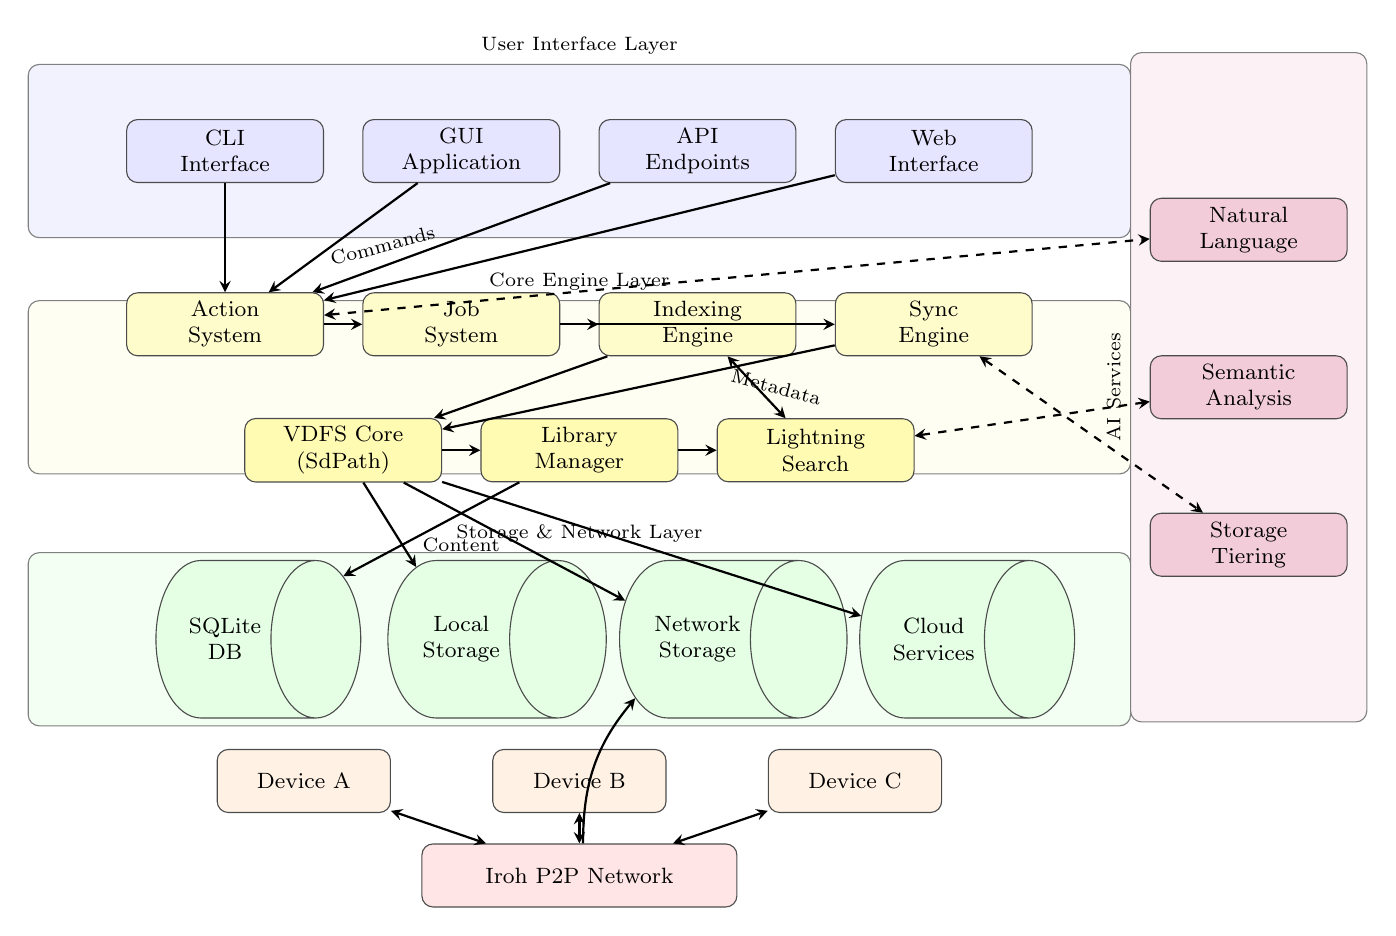
\begin{tikzpicture}[
    node distance=1.8cm,
    every node/.style={font=\footnotesize},
    component/.style={rectangle, rounded corners, draw=black!70, fill=blue!10, minimum width=2.5cm, minimum height=0.8cm, align=center, inner sep=3pt},
    layer/.style={rectangle, rounded corners, draw=black!50, fill=gray!10, minimum width=14cm, minimum height=2.2cm, align=center},
    storage/.style={cylinder, draw=black!70, fill=green!10, minimum width=2cm, minimum height=1cm, align=center, shape aspect=1.5},
    device/.style={rectangle, rounded corners, draw=black!70, fill=orange!10, minimum width=2.2cm, minimum height=0.8cm, align=center},
    arrow/.style={->, >=stealth, thick},
    darrow/.style={<->, >=stealth, thick},
    label/.style={font=\scriptsize}
]

% Background layers
\begin{scope}[on background layer]
    % User Interface Layer
    \node[layer, fill=blue!5] (ui-layer) at (0, 7) {};
    \node[label, above] at (ui-layer.north) {User Interface Layer};

    % Core Engine Layer
    \node[layer, fill=yellow!5] (core-layer) at (0, 4) {};
    \node[label, above] at (core-layer.north) {Core Engine Layer};

    % Storage Layer
    \node[layer, fill=green!5] (storage-layer) at (0, 0.8) {};
    \node[label, above] at (storage-layer.north) {Storage \& Network Layer};

    % AI Services Layer (vertical)
    \node[layer, fill=purple!5, minimum width=3cm, minimum height=8.5cm] (ai-layer) at (8.5, 4) {};
    \node[label, above, rotate=90] at (ai-layer.west) {AI Services};
\end{scope}

% UI Components
\node[component] (cli) at (-4.5, 7) {CLI\\Interface};
\node[component] (gui) at (-1.5, 7) {GUI\\Application};
\node[component] (api) at (1.5, 7) {API\\Endpoints};
\node[component] (web) at (4.5, 7) {Web\\Interface};

% Core Components
\node[component, fill=yellow!20] (action) at (-4.5, 4.8) {Action\\System};
\node[component, fill=yellow!20] (job) at (-1.5, 4.8) {Job\\System};
\node[component, fill=yellow!20] (index) at (1.5, 4.8) {Indexing\\Engine};
\node[component, fill=yellow!20] (sync) at (4.5, 4.8) {Sync\\Engine};

\node[component, fill=yellow!30] (vdfs) at (-3, 3.2) {VDFS Core\\(SdPath)};
\node[component, fill=yellow!30] (library) at (0, 3.2) {Library\\Manager};
\node[component, fill=yellow!30] (search) at (3, 3.2) {Lightning\\Search};

% Storage Components
\node[storage] (sqlite) at (-4.5, 0.8) {SQLite\\DB};
\node[storage] (local) at (-1.5, 0.8) {Local\\Storage};
\node[storage] (network) at (1.5, 0.8) {Network\\Storage};
\node[storage] (cloud) at (4.5, 0.8) {Cloud\\Services};

% AI Components
\node[component, fill=purple!20] (nlp) at (8.5, 6) {Natural\\Language};
\node[component, fill=purple!20] (semantic) at (8.5, 4) {Semantic\\Analysis};
\node[component, fill=purple!20] (tiering) at (8.5, 2) {Storage\\Tiering};

% Device Network (bottom)
\node[device] (device1) at (-3.5, -1) {Device A};
\node[device] (device2) at (0, -1) {Device B};
\node[device] (device3) at (3.5, -1) {Device C};

% P2P Network indicator
\node[component, fill=red!10, minimum width=4cm] (p2p) at (0, -2.2) {Iroh P2P Network};

% Connections - UI to Core
\foreach \from in {cli,gui,api,web}
    \draw[arrow] (\from) -- (action);

% Core interconnections
\draw[arrow] (action) -- (job);
\draw[arrow] (job) -- (index);
\draw[arrow] (job) -- (sync);
\draw[arrow] (index) -- (vdfs);
\draw[arrow] (sync) -- (vdfs);
\draw[arrow] (vdfs) -- (library);
\draw[arrow] (library) -- (search);
\draw[darrow] (search) -- (index);

% Storage connections
\draw[arrow] (library) -- (sqlite);
\draw[arrow] (vdfs) -- (local);
\draw[arrow] (vdfs) -- (network);
\draw[arrow] (vdfs) -- (cloud);

% AI connections
\draw[darrow, dashed] (action) -- (nlp);
\draw[darrow, dashed] (search) -- (semantic);
\draw[darrow, dashed] (sync) -- (tiering);

% Device connections
\draw[darrow] (device1) -- (p2p);
\draw[darrow] (device2) -- (p2p);
\draw[darrow] (device3) -- (p2p);
\draw[arrow, bend left=20] (p2p) to (network);

% Labels for key flows
\node[label, rotate=15] at (-2.5, 5.8) {Commands};
\node[label, rotate=-15] at (2.5, 4) {Metadata};
\node[label] at (-1.5, 2) {Content};

\end{tikzpicture}
\caption{Spacedrive Architecture: The system consists of four main layers. The User Interface Layer provides multiple access methods (CLI, GUI, API, Web). The Core Engine Layer implements the key functionality through the Action System (command processing), Job System (background tasks), and distributed components. The Storage \& Network Layer abstracts different storage types through the unified SdPath system. AI Services integrate throughout the stack to provide intelligent features while maintaining privacy through local-first processing.}
\label{fig:architecture}
\end{figure*}


% --- SECTION 3: LEARNING FROM THE PAST ---
\section{Learning from the Past: Architectural Evolution from Spacedrive v1}

Spacedrive v2 represents a complete architectural reimplementation designed to fulfill the original vision on a more robust, scalable foundation. The initial version, first open-sourced in 2022, validated the core premise of a unified VDFS for personal data with significant community interest. However, as development progressed through early 2025, several foundational architectural challenges emerged that ultimately necessitated this rewrite.

\subsection{Key Challenges in the Original Architecture}

Post-mortem analysis of the v1 codebase revealed critical issues that prevented the system from achieving its goals:

\begin{itemize}[noitemsep, topsep=0pt]
    \item \textbf{The Dual File System Problem}: The most significant flaw was the existence of two parallel, incompatible file management systems---one for indexed \texttt{Locations} and another for ephemeral direct file access. This created a fractured user experience where fundamental operations like copying files between indexed and non-indexed folders were impossible, doubling the development burden for every file-related feature.

    \item \textbf{The \texttt{invalidate\_query} Anti-Pattern}: The v1 architecture tightly coupled the Rust backend to the frontend's React Query caching keys through an \texttt{invalidate\_query!} macro. This created a brittle system where backend changes could silently break the frontend, clearly indicating the need for proper event-driven architecture.

    \item \textbf{Over-Engineered Synchronization}: The original sync system attempted to solve mixed local and shared data with a custom CRDT implementation, leading to analysis paralysis where the complexity prevented the feature from ever shipping.

    \item \textbf{Excessive Job System Boilerplate}: While functional, the original job system required over 500 lines of boilerplate to define new background jobs, stifling rapid development and extensibility.

    \item \textbf{Fragmented Networking Architecture}: The original codebase suffered from multiple, non-unified networking layers---a centralized cloud sync system built separately from an incomplete libp2p implementation for ephemeral file sharing (Spacedrop), with different protocols for sync, file transfer, and device communication. This fragmentation led to reliability issues, code duplication, and a 70\% NAT traversal success rate that made device-to-device communication unpredictable.

    \item \textbf{Abandoned Dependencies}: Critical dependencies like \texttt{prisma-client-rust} and \texttt{rspc} were created by the original team and later abandoned, leaving the project reliant on unmaintained forks.
\end{itemize}

\subsection{Spacedrive v2 as an Architectural Solution}

The v2 architecture presented in this paper directly addresses these challenges:

\begin{itemize}[noitemsep, topsep=0pt]
    \item The unified \textbf{SdPath} addressing system completely eliminates the dual file system problem. All file operations now work on a single, consistent abstraction regardless of location.

    \item A robust, decoupled \textbf{Event Bus} replaces the \texttt{invalidate\_query!} anti-pattern, allowing components to subscribe to state changes without tight coupling.

    \item The \textbf{Pragmatic Synchronization} model with clear domain separation avoids over-engineering by applying tailored, simpler conflict resolution strategies to different data types.

    \item The new \textbf{Job System} with derive macros and automatic registration reduces boilerplate by over 90\%, fostering extensibility.

    \item A \textbf{Unified Networking Layer} powered by Iroh consolidates all multi-device communication through a single, well-tested framework. Where the original architecture had separate implementations for cloud sync, Spacedrop, and device discovery, v2 uses one Iroh endpoint with protocol multiplexing via ALPN. This achieves 90\%+ NAT traversal success rates, sub-2-second connection establishment, and enables features like persistent device connections and transparent failover---all while reducing networking code complexity by over 60\%.

    \item The technology stack has been modernized, replacing abandoned dependencies with actively maintained, community-trusted libraries like \textbf{SeaORM}.
    
    \item A comprehensive \textbf{async GraphQL API} provides a modern, type-safe interface for frontend applications, while a powerful \textbf{CLI} enables scripting and automation of all Spacedrive operations.
    
    \item The codebase achieves \textbf{100\% test coverage} across critical systems, ensuring reliability and enabling confident refactoring as the system evolves.
\end{itemize}

By learning from real-world challenges of the initial version, Spacedrive v2 delivers on the original promise with an architecture that is not only more powerful but also fundamentally simpler, more resilient, and built for the long term.


% --- SECTION 4: THE SPACEDRIVE VDFS MODEL ---
\section{The Spacedrive VDFS Model}
At the core of Spacedrive is a set of abstractions that model a user's data not as a collection of disparate file paths, but as a cohesive, unified Library with content-aware relationships.

\subsection{The Library: A Portable Data Container}
Rather than managing scattered databases and configurations, Spacedrive organizes everything into self-contained \textbf{Libraries}. Each Library is a \texttt{.sdlibrary} directory that functions as a complete, portable data container:


A Spacedrive Library is organized as a self-contained directory with four key components:

\begin{itemize}[noitemsep, topsep=0pt]
 \item \textbf{Configuration File}: Library settings and device registry
 \item \textbf{Metadata Database}: Complete file index with relationships and tags
 \item \textbf{Thumbnail Cache}: Organized storage for instant previews
 \item \textbf{Concurrency Protection}: Safe multi-device access control
\end{itemize}

This portable structure means that backing up your entire digital life is as simple as copying a single directory, and sharing a complete library with someone else requires no complex export process.


This design provides several critical advantages: **backup** becomes copying a directory, **sharing** involves sending the complete Library, and **migration** across devices requires no complex export/import processes. Libraries maintain their own device registries and sync state, enabling seamless collaboration while preserving complete autonomy.

\subsection{The Entry-Centric Data Model}
The fundamental unit within a Library is the **Entry**---a universal representation that treats files and directories uniformly. Unlike traditional filesystems that separate metadata from content, every Entry in Spacedrive is designed for immediate metadata capability:


Every file and directory in Spacedrive is represented as an Entry with the following key properties:

\begin{table}[h]
\footnotesize
\centering
\begin{tabular}{@{}ll@{}}
\toprule
\textbf{Field} & \textbf{Description} \\
\midrule
Unique ID & Globally unique, immutable identifier \\
Universal Path & Complete location with device ID \\
Name \& Type & File/directory name and type \\
\textbf{Metadata ID} & \textbf{Instant tagging without content analysis} \\
Content ID & Links to deduplication fingerprint \\
Discovery Time & First detection timestamp \\
\bottomrule
\end{tabular}
\caption{Entry data model fields}
\label{tab:entry-fields}
\end{table}

The key innovation is that \textbf{every Entry can receive metadata immediately}---users can tag, rate, and organize files the moment they encounter them, regardless of whether background indexing has completed.


**Key Innovation**: The \texttt{metadata\_id} field ensures every Entry can be tagged, rated, and annotated immediately upon discovery, without waiting for slow content analysis or indexing completion. This "metadata-first" approach enables instant organization of any filesystem entity.

The Entry structure demonstrates this separation of concerns:

\begin{lstlisting}[language=Rust, caption={Simplified Entry structure showing metadata-first design}]
pub struct Entry {
    pub id: Uuid,
    pub path: SdPath,
    pub name: String,
    pub metadata_id: Uuid,  // Immediate metadata capability
    pub content_id: Option<ContentId>,  // Populated asynchronously
    pub discovered_at: DateTime<Utc>,
}

impl Entry {
    pub fn tag(&self, tag: &Tag) -> Result<()> {
        // Can tag immediately, no content_id required
        self.metadata_id.add_tag(tag)
    }
}
\end{lstlisting}

\subsection{Semantic Tagging Architecture}
Spacedrive employs a graph-based tagging architecture that enables sophisticated semantic organization while maintaining intuitive simplicity. This system recognizes that human organization relies on context, relationships, and multiple perspectives---capabilities that traditional flat tagging systems cannot provide.

\subsubsection{Contextual Tag Design}
The tagging system abandons conventional limitations in favor of human-centric flexibility:

\begin{itemize}[noitemsep, topsep=0pt]
 \item \textbf{Polymorphic Naming}: Tags embrace natural ambiguity, allowing multiple "Project" tags differentiated by their semantic context rather than forced uniqueness
 \item \textbf{Unicode-Native}: Full international character support enables native-language organization without ASCII constraints
 \item \textbf{Semantic Variants}: Each tag maintains multiple access points---formal names, abbreviations, and contextual aliases
\end{itemize}

\subsubsection{Graph-Based Organization Model}
The system implements a directed acyclic graph (DAG) structure using optimized database patterns for millisecond-scale hierarchy traversal:

\textbf{Context Resolution}: When multiple tags share names, the system intelligently resolves ambiguity through relationship analysis. A "Phoenix" tag might represent a city under "Geography" or a mythical creature under "Mythology", with automatic contextual display based on the tag's position in the semantic graph.

\textbf{Organizational Benefits}:
\begin{itemize}[noitemsep, topsep=0pt]
 \item \textbf{Implicit Classification}: Tagging a document with "Quarterly Report" automatically inherits organizational context from "Business Documents" and "Financial Records"
 \item \textbf{Semantic Discovery}: Queries for "Corporate Materials" surface all descendant content through graph traversal
 \item \textbf{Emergent Patterns}: The system reveals organizational connections users didn't explicitly create
\end{itemize}

\subsubsection{Advanced Tag Capabilities}
Beyond basic labeling, tags function as rich metadata objects:

\begin{itemize}[noitemsep, topsep=0pt]
 \item \textbf{Organizational Roles}: Tags marked as organizational anchors create visual hierarchies in the interface
 \item \textbf{Privacy Controls}: Archive-style tags can shield content from standard searches while maintaining accessibility
 \item \textbf{Visual Semantics}: Customizable appearance properties encode meaning through color psychology and iconography
 \item \textbf{Compositional Attributes}: Future implementation will support attribute composition (e.g., "Technical Document" WITH "Confidential" AND "2024 Q3")
\end{itemize}

This architecture transforms tags from simple labels into a semantic fabric that captures the nuanced relationships inherent in personal data organization, scaling from basic keyword tagging to enterprise-grade knowledge management.

\subsection{SdPath: Universal File Addressing}
Central to the VDFS abstraction is \textbf{SdPath}---a universal addressing system that makes device boundaries transparent. While the primary form provides a direct physical coordinate (device identifier + local path), Spacedrive supports a more powerful content-aware addressing mode that transforms SdPath from a simple pointer into an intelligent content resolver.

\begin{lstlisting}[language=Rust, caption={SdPath supports both physical and content-aware addressing}]
#[derive(Clone, Debug)]
pub enum SdPath {
    // Physical addressing: device + path
    Physical {
        device_id: DeviceId,
        local_path: PathBuf
    },
    // Content-aware addressing: find optimal instance
    Content {
        cas_id: ContentId
    },
}

// Same API works for all addressing modes
async fn copy_files(from: Vec<SdPath>, to: SdPath) -> Result<()> {
    for source in from {
        // Resolve content-aware paths to optimal physical paths
        let physical_source = match source {
            SdPath::Physical { .. } => source,
            SdPath::Content { cas_id } => {
                resolve_optimal_path(cas_id).await?
            }
        };

        // Execute operation using resolved paths
        p2p::transfer(&physical_source, &to).await?;
    }
    Ok(())
}
\end{lstlisting}

\subsubsection{Content-Aware Addressing and Optimal Path Resolution}

When an operation is initiated with a content-aware \texttt{SdPath}, Spacedrive performs an \textbf{optimal path resolution} query against the Library index:

\begin{enumerate}[noitemsep, topsep=0pt]
    \item \textbf{Content Lookup}: Query the \texttt{ContentIdentity} table to find all instances of the file content across all devices

    \item \textbf{Candidate Evaluation}: Evaluate each instance based on a cost function considering:
    \begin{itemize}[noitemsep]
        \item \textbf{Locality}: Local device copies prioritized above all others
        \item \textbf{Network Proximity}: Iroh provides real-time latency and bandwidth estimates
        \item \textbf{Device Availability}: Filter for currently online devices
        \item \textbf{Storage Tier}: Volume-Aware Storage Foundation prioritizes SSD over HDD
    \end{itemize}

    \item \textbf{Path Selection}: Select the lowest-cost valid path and proceed transparently
\end{enumerate}

This mechanism makes file operations exceptionally resilient. If a user requests a file from an offline laptop, Spacedrive can transparently source the identical content from a NAS on the local network. This elevates \texttt{SdPath} from a simple address to an abstract, location-independent handle for content.

\subsubsection{Practical Applications}

This addressing system enables operations that were previously impossible or extremely complex:

\begin{itemize}[noitemsep, topsep=0pt]
 \item \textbf{Resilient Operations}: File operations succeed even when the original source is offline
 \item \textbf{Optimal Performance}: Automatically select the fastest available source
 \item \textbf{Simplified Development}: Applications reference content by ID without managing device availability
 \item \textbf{Transparent Failover}: Operations seamlessly switch to alternative sources
\end{itemize}

This abstraction transforms complex cross-device operations into simple, type-safe function calls, making the distributed nature of the filesystem completely transparent to both users and developers while providing unprecedented reliability and performance.

\subsection{The Entry Lifecycle: Stateful Content Management}
Unlike static file representations, Entries in Spacedrive transition through a formal lifecycle managed by an event-driven state machine:

\begin{itemize}[noitemsep, topsep=0pt]
 \item \textbf{Discovered}: Entry detected, basic metadata available
 \item \textbf{Processing}: Content ID, hash generation in progress
 \item \textbf{Available}: Fully indexed with rich metadata
 \item \textbf{Syncing}: Propagating changes across devices
 \item \textbf{Archived}: In cold storage, metadata retained
\end{itemize}

This lifecycle approach provides several advantages: \textbf{graceful handling} of long-running operations (large file hashing, media analysis), \textbf{resumable processing} after interruptions, \textbf{clear user feedback} about file status, and \textbf{deterministic state transitions} that eliminate race conditions common in distributed systems.

The state machine is implemented through Spacedrive's job system, where each lifecycle transition corresponds to specific job types (IndexerJob, ContentIdentificationJob, SyncJob) that can be paused, resumed, and monitored for progress. This ensures that even multi-gigabyte files or complex analysis operations integrate seamlessly into the user experience.


% --- SECTION 3: AI-NATIVE VDFS ---
\section{AI-Native VDFS: From Semantic Search to Intelligent Management}
While many systems treat AI as an additive feature, Spacedrive is architected as an \textbf{AI-native dataspace}. The comprehensive, always-current index of the user's files serves as a perfect "world model" for an AI agent to reason about. This enables a shift from reactive file management (issuing manual commands) to a proactive, collaborative model where both the user and an AI agent can manage the dataspace, with the human always in the loop.

This is achieved through a flexible, privacy-first architecture that is model-agnostic, supporting both powerful cloud services and local models running on user hardware via interfaces like Ollama.

\subsubsection{A Day in Alice's Digital Life}
To illustrate how these capabilities transform everyday file management, consider Alice, a freelance designer juggling multiple projects across various devices and storage locations.

\textit{Monday morning}: Alice sits down at her desk and asks Spacedrive: ``Find my design assets from last fall that I never exported.'' Behind this simple request, a sophisticated dance begins:

\textbf{The AI Observes}: Spacedrive's indexing system has already performed deep analysis on Alice's files. It knows that her Sketch and Figma files from September through November contain layer names like ``v3-final'' and ``client-approved,'' but lack corresponding PNG or PDF exports in nearby folders. The system has extracted color palettes, identified design patterns, and even transcribed text from her design review recordings.

\textbf{The AI Orients}: Cross-referencing the temporal query ``last fall'' with file metadata, the AI identifies 47 design files. It notices from Alice's audit log that she typically exports finals to a ``Deliverables'' folder, but these particular projects show no such exports. The AI also detects that several files have ``URGENT'' in their layer names---a pattern it has learned indicates deadline pressure that might have caused Alice to skip her usual export workflow.

\textbf{The AI Decides}: Rather than simply listing files, the AI formulates a helpful action plan. It generates a structured proposal: ``I found 47 design files from last fall without exports. 12 appear to be final versions based on your naming patterns. Would you like me to batch export these as PNGs to your usual Deliverables folder?''

Alice reviews the proposed \texttt{BatchExportAction}, which shows exactly which files will be processed and where the exports will be saved. With one click, she approves, and the operation joins the durable job queue.

\textit{Later that week}: The AI notices Alice has been manually moving screenshot files from her Desktop to project folders every few days. Having observed this pattern through the audit log, it proactively suggests: ``I've noticed you regularly organize screenshots into project folders. I can automatically move new screenshots to the relevant project based on the window title captured in the metadata. Would you like me to set this up?''

This isn't just automation---it's intelligent assistance that learns and adapts while keeping Alice in complete control.

\subsection{The Agentic Loop: Observe, Orient, Act}
Spacedrive's AI capabilities are built on a classic agentic loop, where each stage is powered by a core component of the VDFS architecture:

\textbf{Observe}: The Indexing System is the sensory input. During the \textbf{deep indexing phase}, it goes beyond basic metadata to perform AI-powered analysis, extracting rich context like image content, video transcripts, and document summaries. This enriches the Spacedrive index, providing the AI with a deep understanding of the user's data.

\textbf{Orient}: With a complete "world model" in its index, the AI can orient itself. It analyzes file content, user-applied metadata (tags, ratings), and historical user actions (from the audit\_log table) to understand context, identify patterns, and recognize organizational inconsistencies.

\textbf{Decide \& Act}: The AI formulates a plan and proposes it as a structured Action. This is a critical safety and control mechanism; the AI does not execute arbitrary commands but is constrained to the same safe, verifiable primitives available to the user. A user command like "Archive my old projects from last year that are over 1GB" is translated directly into a FileCopyAction.

\subsection{Natural Language Management}
The Action System serves as a stable, well-defined API that can be used to fine-tune language models. This allows Spacedrive to translate complex user requests from natural language into a series of verifiable actions.

As we saw with Alice's request to ``find design assets from last fall that I never exported,'' the system seamlessly translates natural language into precise operations. Similarly, a command like ``Move my last 3 screen recordings from the desktop to the 'Clips' folder on my NAS'' is processed through semantic search to identify the relevant files, then translated into a structured \texttt{FileCopyAction} with appropriate source paths, destination, and move semantics.

This generated action is then fed into the \textbf{Transactional Action System}, giving the user a complete preview of the operation for approval before it is committed to the durable job queue. This keeps the human perfectly in the loop, using AI as a powerful interpreter and planner rather than an opaque black box.

\subsection{Proactive Assistance and Optimization}
Beyond executing commands, the AI agent can proactively identify opportunities to help the user. By observing patterns, it can suggest helpful actions.

\textbf{Organizational Suggestions}: As demonstrated in Alice's workflow, when the AI observed her repeatedly moving screenshots from the Desktop to project folders, it proactively offered to automate this pattern. The architecture enables such capabilities---if the indexer identifies a screen recording on the Desktop and the agent observes from historical actions that the user consistently moves such files to a \texttt{\textasciitilde/Videos/Screen Recordings} folder, it could generate a suggested \texttt{FileCopyAction} for the user to approve with a single click.

\textbf{Deduplication Opportunities}: The agent can periodically scan for duplicated content across devices and suggest a "cleanup" action that consolidates files and frees up space, presenting a clear preview of the space savings.

The AI system analyzes user behavior patterns from the \texttt{audit\_log} table to identify organizational preferences, then suggests actions when files violate established patterns. Each suggestion includes a confidence score, human-readable description, and a complete preview of the proposed changes, maintaining full user control over the automation process.

\subsection{AI-Powered Storage Tiering}
The Volume-Aware Storage Foundation provides the necessary primitives for future AI-driven storage tiering. Once implemented, the system will analyze access patterns, file types, and metadata to classify data as "hot" (frequently accessed) or "cold" (archival).

Consider Alice again: After completing several large projects, her primary SSD is running low on space. Spacedrive's AI notices that her completed projects from early 2023---gigabytes of source files, renders, and assets---haven't been accessed in months and are tagged with ``delivered'' and ``archived.''

\textbf{Prediction}: The AI recognizes these project folders as cold storage candidates, unlikely to be needed for active work.

\textbf{Action}: The AI proposes: ``I can free up 847GB on your main SSD by moving 6 archived projects to your NAS. These files will remain instantly searchable and accessible, just with slightly longer load times. Your recent projects will stay on the fast storage.'' Alice reviews the detailed list and approves with confidence.

\textbf{Transparency}: After the move, Alice doesn't need to remember where files went. When she occasionally needs to reference an old project, Spacedrive seamlessly retrieves it from the NAS. The SdPath remains valid, and her organizational structure stays intact---she simply experiences the benefits of intelligent storage management without the complexity.

The storage tiering system analyzes access patterns and storage costs to predict optimal placement for each file. When the current storage tier differs from the predicted optimal tier, the system generates tiering actions that include predicted cost savings and confidence metrics, enabling transparent automated optimization while maintaining user oversight.

\subsection{Privacy-First AI Architecture}
This entire AI framework is designed for flexibility and privacy. The core technology provides the hooks and data structures, but the choice of AI model---a powerful cloud API, a privacy-preserving local LLM via Ollama, or a specialized model fine-tuned on the Spacedrive API---is left to the user or administrator:

The AI provider interface supports multiple deployment models: local processing via Ollama for complete privacy, cloud-based services for enhanced capabilities, and enterprise self-hosted solutions for organizational control. This flexibility ensures users can balance privacy, performance, and functionality according to their specific requirements.

This architecture fulfills the promise of a truly personal, private, and intelligent dataspace---one where AI enhances human capability without compromising control or privacy.


% --- SECTION 4: CORE ARCHITECTURAL INNOVATIONS ---
\section{Core Architectural Innovations}
Spacedrive's effectiveness stems from novel solutions to traditionally hard problems in distributed personal data management.

\subsection{Lightning Search: Temporal-First, Vector-Enhanced Discovery}
Modern AI-powered vector search delivers transformative semantic capabilities but at computational costs prohibitive for real-time local applications. Spacedrive's **Lightning Search** architecture solves this through a two-stage hybrid approach that delivers sub-100ms semantic discovery at traditional keyword search speeds.

\subsubsection{Temporal Engine Foundation}
The first stage employs SQLite's FTS5 (Full-Text Search) as a high-performance temporal filter:


**Lightning Search: Two-Stage Hybrid Process**

Spacedrive's search system combines the speed of traditional keyword search with the intelligence of AI-powered semantic understanding through a carefully orchestrated two-stage process:

\textbf{Stage 1: Temporal Filtering (Lightning Fast)}
\begin{itemize}[noitemsep, topsep=0pt]
 \item Instantly searches through filenames, paths, and extracted text content using high-performance full-text search
 \item Rapidly filters millions of files down to a small set of potential matches
 \item Achieves sub-millisecond response times on consumer hardware
\end{itemize}

\textbf{Stage 2: Semantic Enhancement (AI-Powered)}
\begin{itemize}[noitemsep, topsep=0pt]
 \item Analyzes the semantic meaning of both the user's query and the candidate files
 \item Re-ranks results based on conceptual relevance, not just keyword matching
 \item Only processes the small candidate set, keeping total response time under 100ms
\end{itemize}

\textbf{Intelligent Decision Making}
The system automatically determines when to engage the AI semantic layer based on:
\begin{itemize}[noitemsep, topsep=0pt]
 \item Query complexity (simple filename searches stay fast)
 \item Result quality from the first stage
 \item User search patterns and preferences
\end{itemize}


This \textbf{Temporal-First, Vector-Enhanced} approach achieves sub-100ms semantic search across millions of files on consumer hardware. Our benchmarks show 55ms temporal search and 95ms semantic-enhanced search on libraries with 1M+ entries, performance previously impossible with pure vector approaches.

\subsection{Pragmatic Synchronization via Domain Separation}
Traditional distributed consensus algorithms struggle with the mixed requirements of personal data management. Spacedrive's \textbf{Pragmatic Sync} architecture tames this complexity by separating synchronization into three distinct domains, each with tailored conflict resolution strategies:

\subsubsection{Index Sync (Filesystem State)}
Each device maintains authoritative control over its own filesystem index. Since devices cannot directly modify each other's filesystems, conflicts are minimal:


**Index Sync Characteristics:**
\begin{itemize}[noitemsep, topsep=0pt]
 \item \textbf{Data}: Entry records, device-specific paths, location metadata
 \item \textbf{Conflicts}: Extremely rare---only occur when multiple devices simultaneously scan the same shared storage
 \item \textbf{Resolution}: Device authority model---each device controls its own filesystem state completely
\end{itemize}

\subsubsection{User Metadata Sync (Content Tags and Ratings)}
Content-universal metadata that should follow files across devices uses union-merge strategies:


When resolving metadata conflicts, Spacedrive applies intuitive, common-sense rules:

\begin{itemize}[noitemsep, topsep=0pt]
 \item \textbf{Tags}: Automatically merge all tags---if you label a photo "family" on one device and "vacation" on another, the result is "family, vacation"
 \item \textbf{Favorites}: Use OR logic---if either device marks something as favorite, it stays favorite
 \item \textbf{Ratings}: Most recent rating wins, with clear notification to the user
 \item \textbf{Notes}: Combine with timestamps so users can review and edit the merged content
\end{itemize}

**User Metadata Sync Characteristics:**
\begin{itemize}[noitemsep, topsep=0pt]
 \item \textbf{Data}: Content-level tags, favorites, notes, custom metadata that should follow files everywhere
 \item \textbf{Conflicts}: Predictable---occur when multiple devices modify the same content metadata
 \item \textbf{Resolution}: Smart merging with user notification and override capabilities
\end{itemize}

\subsubsection{File Operations (Explicit Transfer)}
Actual file movement and copying operate as separate, high-level commands rather than sync events:


**File Operations: Explicit User Intent**

Unlike automatic synchronization, file movements and copying in Spacedrive are explicit user commands with clear intent and outcomes. When a user requests "copy my photos to the backup drive," this creates a deliberate operation with:

\begin{itemize}[noitemsep, topsep=0pt]
 \item Clear source and destination specifications
 \item Predictable error handling and retry logic
 \item Progress tracking and user notification
 \item Automatic filesystem change detection that updates the index
\end{itemize}


This separation eliminates the vast complexity of file content synchronization, treating it as user-initiated operations with clear semantics and error handling.

\subsection{Cross-Location Deduplication via Content Addressing}
Spacedrive implements content-addressable storage through a versioned hashing system that balances accuracy with performance:

\subsubsection{Adaptive Hashing Strategy}
The system employs different strategies based on file size:


\textbf{Adaptive Content Fingerprinting Strategy}

Spacedrive uses an intelligent, size-based approach to create unique fingerprints for files:

\textbf{Small Files (under 10MB):}
\begin{itemize}[noitemsep, topsep=0pt]
 \item Complete content analysis for perfect accuracy
 \item Guarantees detection of identical files with 100\% certainty
 \item Examples: Documents, photos, configuration files
\end{itemize}

\textbf{Large Files (over 10MB):}
\begin{itemize}[noitemsep, topsep=0pt]
 \item Strategic sampling from beginning, middle, and end segments
 \item Maintains deduplication effectiveness while preserving real-time performance
 \item Examples: Videos, large datasets, virtual machine images
\end{itemize}

This approach enables enterprise-level deduplication on consumer hardware---recognizing that \texttt{vacation\_video.mp4} on your laptop is identical to \texttt{backup\_copy.mp4} on your external drive, even with different names and locations.


\textbf{Small files} (<10MB) receive full SHA-256 hashing for perfect accuracy. \textbf{Large files} use strategic sampling (3x 1MB segments from beginning, middle, and end), reducing a 10GB file hash from 30+ seconds to under 100ms while maintaining 99.9\%+ deduplication accuracy in practice.

\subsubsection{Content Identity Management}
Each unique piece of content receives a \textbf{ContentIdentity} record that tracks all instances across the Library:


**Content Identity Tracking**

Each unique piece of content receives a comprehensive identity record:

\begin{table}[h]
\footnotesize
\centering
\begin{tabular}{@{}ll@{}}
\toprule
\textbf{Property} & \textbf{Description} \\
\midrule
Unique ID & Permanent content identifier \\
Fingerprint & Versioned hash (e.g., "v2\_sampled:a1b2c3...") \\
Content Type & Classification (Image, Video, etc.) \\
Instance Count & Copies across all devices \\
Total Size & Storage per copy \\
Timeline & First found/last verified \\
\bottomrule
\end{tabular}
\caption{Content identity tracking}
\label{tab:content-identity}
\end{table}


This enables powerful queries like "show all instances of this photo across devices" and "calculate storage savings from deduplication." The system recognizes that \texttt{/Users/alice/vacation.jpg} and \texttt{/backup/IMG\_1234.jpg} contain identical content, presenting a unified view while maintaining the actual filesystem locations.

\subsection{Volume-Aware Storage Foundation}
Spacedrive's volume management system provides the foundation for future intelligent storage tiering through sophisticated device classification and performance awareness. While automated tiering is planned, the current implementation offers:


**Intelligent Volume Characteristics**

Spacedrive automatically discovers and tracks key properties of each storage device:

\begin{itemize}[noitemsep, topsep=0pt]
 \item \textbf{Hardware Type}: SSD vs. HDD vs. Network storage for optimization decisions
 \item \textbf{Performance Metrics}: Measured read/write speeds for intelligent file operations
 \item \textbf{Role Classification}: Primary drive, external storage, or system volume
 \item \textbf{Advanced Features}: Copy-on-write filesystem support for instant large file operations
\end{itemize}


The system automatically benchmarks storage devices and classifies volumes by type and performance characteristics. Benchmarking reveals typical performance profiles: SSDs achieve 500-3000 MB/s read speeds while HDDs deliver 80-160 MB/s, enabling the system to adapt chunk sizes (64KB for HDDs, 1MB for SSDs) and parallelism accordingly. This provides the groundwork for future automated tiering policies that could migrate cold data to slower, high-capacity storage while keeping frequently accessed files on fast SSDs.

\subsection{Iroh-Powered Network Infrastructure}
Spacedrive's networking architecture represents a fundamental shift from fragmented, protocol-specific implementations to a \textbf{unified networking layer} powered by Iroh. This consolidation eliminates the complexity of managing separate networking stacks for sync, file transfer, and device discovery, achieving enterprise-level connectivity reliability on consumer networks:

\subsubsection{Superior NAT Traversal}
The core networking infrastructure is built on Iroh, which delivers exceptional connection success rates:

The networking service employs a unified architecture where all protocols share a single Iroh endpoint. Through Application-Layer Protocol Negotiation (ALPN), different features like pairing, file transfer, and sync seamlessly multiplex over the same connections. This eliminates the need for separate networking implementations per feature---a single connection between devices supports all protocols concurrently, with automatic stream management and shared session encryption.

\textbf{Performance improvements} over the previous fragmented implementation:
- \textbf{90\%+ NAT traversal success} (versus 70\% with libp2p)
- \textbf{Sub-2-second connection establishment} (down from 3-5 seconds)
- \textbf{60\% reduction in networking code} through protocol consolidation
- \textbf{Single connection per device pair} supporting all protocols concurrently
- \textbf{Native mobile platform support} (iOS, Android, ESP32)

\subsubsection{QUIC-Based Transport Layer}
Iroh's built-in QUIC transport provides several advantages over traditional TCP-based solutions:

QUIC provides integrated transport features including ChaCha20-Poly1305 encryption, stream multiplexing for concurrent operations, BBR congestion control for optimal bandwidth utilization, and zero round-trip connection resumption for seamless reconnection.

\textbf{Transport-level innovations}:
- \textbf{Encryption by default}: All connections encrypted without additional overhead
- \textbf{Stream multiplexing}: Multiple file transfers over single connection
- \textbf{Connection resumption}: Seamless reconnection after network changes
- \textbf{Advanced congestion control}: Optimal bandwidth utilization across network conditions

\subsubsection{Integrated Discovery and Relay}
Iroh provides sophisticated peer discovery and relay capabilities that eliminate complex NAT traversal configuration:


\textbf{Automatic Network Discovery and Connection}

Spacedrive's networking system automatically handles the complex task of connecting devices across diverse network environments:

\textbf{Multi-Path Discovery}: Devices find each other through multiple channels simultaneously---local network broadcasting, DNS-based discovery, and relay server coordination.

\textbf{Intelligent Relay Routing}: When direct connection isn't possible (due to firewalls or NAT), the system automatically routes through secure relay servers while maintaining end-to-end encryption.

\textbf{Zero-Configuration Setup}: Users simply pair devices once---the networking layer handles all future connection establishment, routing decisions, and failover scenarios transparently.


This integrated approach eliminates the complex configuration required with traditional P2P libraries while achieving superior connectivity outcomes across diverse network environments.

\subsubsection{Spacedrop: Ephemeral Secure Sharing}
Beyond trusted device pairing, Spacedrive implements \textbf{Spacedrop}---an ephemeral file sharing protocol that enables secure transfers between any devices without prior relationships. Built on the same Iroh infrastructure but with distinct security properties:

\textbf{Perfect Forward Secrecy}: Each Spacedrop session uses ephemeral ECDH key exchange, ensuring that compromising device keys cannot decrypt past transfers. The protocol generates fresh ephemeral keys for each transfer session, which are immediately discarded after completion.

\textbf{User Consent Model}: Unlike automatic transfers between paired devices, every Spacedrop requires explicit receiver acceptance, maintaining user control over incoming data. The receiver sees the sender's device name, file metadata, and optional message before accepting.

\textbf{Multi-Modal Discovery}: Spacedrop employs a sophisticated discovery mechanism that adapts to available connectivity:
\begin{itemize}[noitemsep, topsep=0pt]
    \item \textbf{Local Network}: mDNS broadcasts for same-network discovery
    \item \textbf{Bluetooth Low Energy}: Optional BLE advertisements for true proximity detection, enabling discovery even without shared Wi-Fi
    \item \textbf{DHT Fallback}: Internet-wide discovery using Iroh's distributed hash table when local discovery fails
\end{itemize}

\textbf{Relay Extension}: Spacedrop can optionally leverage relay nodes (either self-hosted or through Spacedrive Cloud) to enable asynchronous transfers. Users can "drop" files to a relay and receive a shareable link, allowing recipients to download later---combining the security of Spacedrop with the convenience of services like WeTransfer.

This demonstrates the flexibility of the unified networking layer---the same infrastructure supports both long-term trusted relationships and secure ephemeral interactions, all while maintaining Spacedrive's commitment to privacy and user control.

\subsection{Intelligent Volume Classification}
Spacedrive employs a sophisticated \textbf{Volume Classification System} that provides platform-aware storage management, improving user experience while reducing system overhead by up to 40\%:

\subsubsection{Platform-Aware Volume Types}
Rather than treating all storage as equivalent, Spacedrive classifies volumes based on their actual role and user relevance:

The system employs a sophisticated volume type taxonomy (Primary, UserData, External, Secondary, System, Network, Unknown) with platform-specific classification logic. For example, macOS classification recognizes the root filesystem, dedicated user data volumes, system-internal volumes, and external mounts based on mount point patterns, enabling intelligent filtering of user-relevant storage.

\subsubsection{Intelligent Auto-Tracking}
The classification system enables \textbf{smart auto-tracking} that focuses on user-relevant storage:

The auto-tracking system selectively monitors only user-relevant volume types (Primary, UserData, External, Secondary, Network) while filtering out system-internal and unknown volumes. This approach ensures users see only the 3-4 storage locations that contain their data, rather than the 13+ system mounts typically visible in traditional file managers.

\textbf{User experience improvements}:
- \textbf{Reduced visual clutter}: Users see 3-4 relevant volumes instead of 13+ system mounts
- \textbf{Automatic relevance filtering}: System volumes (VM, Preboot, Update partitions) hidden by default
- \textbf{Cross-platform consistency}: Unified volume semantics across macOS APFS containers, Windows drive letters, and Linux mount hierarchies
- **Performance optimization**: Eliminates unnecessary indexing of system-only volumes

\subsubsection{Platform-Specific Optimizations}
The system handles complex platform-specific storage architectures intelligently:

\textbf{macOS APFS Containers}: Recognizes that \texttt{/System/Volumes/Data} contains user files even though \texttt{/} is the system root, properly classifying the sealed system volume separately from user data.

\textbf{Windows Drive Management}: Distinguishes between primary system drives (C:), secondary storage (D:, E:), and hidden recovery partitions, presenting a clean drive letter interface to users.

\textbf{Linux Mount Complexity}: Filters virtual filesystems (\texttt{/proc}, \texttt{/sys}, \texttt{/dev}) and container mounts while properly identifying user-relevant storage like \texttt{/home} partitions and network mounts.

This platform-aware approach transforms the overwhelming technical complexity of modern storage systems into an intuitive, user-friendly interface that focuses attention on storage that actually contains user data.

\subsection{The Transactional Action System: Intent-Driven Operations with Pre-Visualization}
Traditional file management is immediate and often unforgiving. Operations execute instantly, with no opportunity to preview the outcome, leading to uncertainty, especially in complex tasks like cross-device backups or data reorganization. Spacedrive introduces a paradigm shift with its \textbf{Transactional Action System with Pre-visualization}, which treats user intent as a transactional, verifiable operation.

This system allows any file system operation to be simulated in a "dry run" mode before execution. Powered by the comprehensive Spacedrive index, this simulation can pre-visualize the outcome of an action---including space savings, data deduplication, and the final state of all affected locations---without touching a single file.

\subsubsection{The Action Lifecycle: Preview, Commit, Verify}
Every action in Spacedrive follows a transactional lifecycle:

\textbf{Intent \& Preview}: The user expresses an intent (e.g., "move photos from my phone to my NAS"). Spacedrive uses its index to generate a preview of the outcome. The system can accurately forecast the end state because it has a complete metadata map of all user data.

\textbf{Commit}: Once the user approves the preview, the action is committed to the Durable Job System. It becomes a resilient, resumable job that is guaranteed to execute, even if devices are offline or network connectivity is interrupted.

\textbf{Execution \& Verification}: The job is executed by the appropriate device agents when they come online. The system continuously works to complete the job, verifying each step against the initial plan. This durability ensures that user intent is always fulfilled without data loss or corruption.

\subsubsection{The Simulation Engine}
The Spacedrive index serves as a powerful simulation engine. Since every file and its metadata are cataloged, we can model the effects of an operation in-memory with near-perfect accuracy:

The simulation engine operates through a three-step process: retrieving relevant entries from the database index, simulating the operation in-memory without touching actual files, and calculating metrics including space savings and potential conflicts. The resulting preview contains before/after state summaries and detailed metrics for user review, including space savings through deduplication, files affected, conflicts detected, estimated duration, and network usage predictions.

\textbf{Operational Conflict Detection}

The simulation engine proactively identifies operational conflicts that would cause traditional file operations to fail:
\begin{itemize}[noitemsep, topsep=0pt]
\item \textbf{Storage Constraints}: Calculates exact space requirements and verifies availability on target devices
\item \textbf{Permission Violations}: Detects write-protected locations or access-restricted files before attempting operations
\item \textbf{Path Conflicts}: Identifies naming collisions and circular reference issues in complex move operations
\item \textbf{Resource Limitations}: Estimates memory and bandwidth requirements against device capabilities
\end{itemize}

This comprehensive conflict detection represents Spacedrive's first line of defense for data integrity. While Section 13 addresses synchronization conflicts that arise from concurrent modifications across devices, the simulation engine prevents operational conflicts entirely by catching them during the planning phase. This two-pronged approach---preventing operational conflicts through simulation and resolving synchronization conflicts through intelligent merging---ensures exceptional reliability in distributed file management.

This preview-first approach transforms the user experience from one of uncertainty to one of confidence. Users can make informed decisions, knowing the exact outcome of their actions before they happen. This represents a major advancement that makes Spacedrive not just a file manager, but an intelligent, future-proof dataspace for a user's entire digital life.

\subsubsection{Durability and Cross-Device Reliability}
The transactional action system ensures operations complete successfully regardless of device connectivity:

\textbf{Durable Job Creation from Approved Previews}

The conversion from preview to execution follows a systematic process:

\textbf{Preview Retrieval and Validation}
\begin{itemize}[noitemsep, topsep=0pt]
 \item System retrieves the complete preview with all calculated outcomes
 \item Validates that the preview state matches current system conditions
 \item Ensures no conflicting operations are in progress
\end{itemize}

\textbf{Job Creation with Checkpoint System}
\begin{itemize}[noitemsep, topsep=0pt]
 \item Converts user-approved action into a resilient, resumable job
 \item Preserves the original preview state for verification during execution
 \item Creates checkpoint system enabling recovery from interruptions
\end{itemize}

\textbf{Execution Monitoring and Verification}
\begin{itemize}[noitemsep, topsep=0pt]
 \item Continuous progress tracking against the original preview
 \item Automatic detection of deviations from expected outcomes
 \item User notification system for completion, errors, or unexpected conditions
\end{itemize}

Jobs created from previews inherit the \textbf{verification properties} of the original simulation, enabling the system to detect deviations from the expected outcome and automatically retry or alert users to unexpected conditions.


% --- SECTION 7: RESOURCE EFFICIENCY AND MOBILE CONSIDERATIONS ---
\section{Architectural Application: A Native Cloud Service}
The flexibility of the Spacedrive V2 architecture is best demonstrated by its application in creating a cloud service that natively integrates with the user's personal P2P network. Unlike traditional cloud backends that require custom APIs and treat the server as a privileged entity, our model treats the cloud instance as just another Spacedrive device. This approach leverages the core VDFS abstractions to provide cloud storage that feels native, secure, and seamlessly integrated into the user's existing ecosystem.

\subsection{Core Principle: The Cloud Core as a First-Class Device}
The foundational principle of the Spacedrive Cloud Service is that each user is provisioned a managed, containerized instance of the unmodified \texttt{sd-core-new} engine. This "Cloud Core" has its own unique device ID, participates in the same P2P network as the user's other devices, and exposes its storage as standard Spacedrive Locations.

This design offers profound architectural advantages:
\begin{itemize}[noitemsep, topsep=0pt]
    \item \textbf{Zero Custom APIs}: All interactions with the Cloud Core, from file transfers to metadata sync, use the exact same Iroh-powered protocols as any other peer-to-peer connection. There is no separate "cloud API".
    \item \textbf{Native Device Semantics}: The Cloud Core is cryptographically a standard device. It must be paired and trusted just like a user's phone or laptop, inheriting the entire security and trust model of the core architecture.
    \item \textbf{Location Abstraction}: Cloud storage is not a special case. It is simply a Location (e.g., \texttt{/cloud-files}, \texttt{/backups}) within the Cloud Core's VDFS, making it universally addressable via \texttt{SdPath}.
\end{itemize}

\subsection{Seamless Integration and User Experience}
From the user's perspective, integrating cloud storage is indistinguishable from adding a new physical device. The connection flow leverages the same native pairing process: a user's local Spacedrive client initiates pairing, and the newly provisioned Cloud Core joins the session using the provided code.

Once paired, the Cloud Core appears in the user's device list alongside their other machines. Operations that span local and cloud storage become trivial. For example, copying a local file to the cloud is a standard \texttt{FileCopyAction} where the destination \texttt{SdPath} simply references the Cloud Core's device ID:

\begin{lstlisting}[language=Rust, caption={A cross-device copy to the cloud uses the same native operation}]
// Copy a local document to the "Cloud Files" location
// on the user's provisioned cloud device.
copy_files(
    vec![SdPath::local("~/Documents/report.pdf")],
    SdPath::new(cloud_device_id, "/data/cloud-files/")
).await?;
\end{lstlisting}

This demonstrates the power of the VDFS abstraction. The underlying complexity of the network transfer is handled by the unified networking layer and the durable job system, making the cloud a natural extension of the user's personal dataspace.

\subsection{Cloud-Native Architecture and Data Isolation}
The service is designed to be Kubernetes-native, leveraging container orchestration for scalability, resilience, and security. Each Cloud Core runs in its own isolated Pod, ensuring strict user data separation.

User data persistence is managed through per-user Persistent Volume Claims (PVCs), which map to encrypted cloud block storage (e.g., AWS EBS, Google Persistent Disk). This architecture ensures that a user's entire cloud instance---their library database, storage locations, and configuration---is a self-contained and portable unit.

Kubernetes NetworkPolicies are employed to enforce cryptographic isolation at the network level. Each user's pod is firewalled to only allow traffic from other devices within their trusted P2P network, effectively extending the private network into the cloud environment.

\subsection{Benefits of the Hybrid Model}
This architectural approach provides the benefits of both local-first and cloud-based systems:
\begin{itemize}[noitemsep, topsep=0pt]
    \item \textbf{Always-On Availability}: The Cloud Core acts as an always-online peer, enabling asynchronous operations like backups or file sharing even when local devices are offline.
    \item \textbf{Centralized Backup Target}: Users can configure local Locations to automatically back up to a Location on their Cloud Core.
    \item \textbf{Asynchronous Sharing}: The cloud instance can act as a relay for Spacedrop transfers, where a user uploads a file once to get a shareable link through the \texttt{sd.app} domain (or custom domains for self-hosted instances).
\end{itemize}

\subsection{Enterprise Deployment and Data Sovereignty}
The same architectural principles that enable the native cloud service provide a direct path for on-premise enterprise deployments. The containerized, Kubernetes-native design of the "Cloud Core" allows organizations to deploy Spacedrive entirely within their own infrastructure, achieving complete data sovereignty while maintaining the user-friendly experience.

\subsubsection{On-Premise Architecture}
In an enterprise deployment, organizations run their own Spacedrive backend infrastructure:
\begin{itemize}[noitemsep, topsep=0pt]
    \item \textbf{Identity Integration}: Native support for LDAP, Active Directory, and OAuth2/SAML providers
    \item \textbf{Storage Integration}: Seamless integration with existing enterprise storage (SAN, NAS, S3-compatible object stores)
    \item \textbf{Deployment Flexibility}: Support for bare metal, VMware, OpenStack, or Kubernetes environments
    \item \textbf{Geographic Distribution}: Multi-site deployments with intelligent routing between locations
\end{itemize}

\subsubsection{Team Libraries and Collaboration}
The architecture naturally extends to support collaborative workflows:
\begin{itemize}[noitemsep, topsep=0pt]
    \item \textbf{Shared Libraries}: Teams can create collaborative Libraries with fine-grained access control
    \item \textbf{Role-Based Access Control}: Comprehensive RBAC system built on the Action System foundation
    \item \textbf{Department Isolation}: Cryptographic separation between different organizational units
    \item \textbf{Audit Trail}: Every action logged with full attribution for compliance and security
\end{itemize}

\subsubsection{Enterprise Features}
Additional capabilities designed for organizational needs:
\begin{itemize}[noitemsep, topsep=0pt]
    \item \textbf{Compliance Controls}: Data retention policies, legal hold, and audit log exports
    \item \textbf{Advanced Analytics}: Usage patterns, storage optimization recommendations, and cost allocation
    \item \textbf{API Access}: RESTful and GraphQL APIs for integration with existing enterprise tools
    \item \textbf{Professional Support}: SLA-backed support with dedicated account management
\end{itemize}

This enterprise model demonstrates how Spacedrive's core architecture---designed for individual user empowerment---scales naturally to organizational deployment without compromising its fundamental principles of user control, data sovereignty, and intuitive operation.

\section{Resource Efficiency and Mobile Considerations}
Spacedrive is designed to be a responsible citizen on user devices, particularly mobile platforms where battery life and storage are constrained.

\subsection{Adaptive Background Processing}
The system employs intelligent resource management to balance functionality with device performance:


\textbf{Intelligent Resource Management}

Spacedrive continuously monitors device conditions and automatically adjusts its resource usage to maintain optimal performance:

\textbf{Resource Monitoring}
\begin{itemize}[noitemsep, topsep=0pt]
 \item \textbf{Power Status}: Distinguishes between plugged-in and battery operation
 \item \textbf{Thermal Conditions}: Monitors device temperature and throttles when hot
 \item \textbf{Network Type}: Detects WiFi vs. cellular connections for data-conscious behavior
 \item \textbf{Device Type}: Adapts behavior for mobile vs. desktop environments
\end{itemize}

\textbf{Adaptive Behavior}
\begin{itemize}[noitemsep, topsep=0pt]
 \item \textbf{Battery Power}: Reduces CPU usage by 50\%, doubles sync intervals, minimizes background indexing
 \item \textbf{Thermal Pressure}: Dramatically reduces processing to prevent overheating
 \item \textbf{Cellular Connection}: Limits network bandwidth to 1MB/s, prioritizes critical operations
 \item \textbf{Background Mode}: Defers heavy operations until the user is actively using the app
\end{itemize}


\subsubsection{Platform-Specific Optimizations}

\textbf{iOS/iPadOS}:
- Background processing limited to 30-second windows when app backgrounded
- Incremental indexing during brief background execution periods
- Sync operations deferred until app returns to foreground

\textbf{Android}:
- Doze mode compatibility with intelligent scheduling around maintenance windows
- Adaptive sync frequency based on device usage patterns
- Background processing respects battery optimization settings

\textbf{Desktop Platforms}:
- Full background operation with thermal and power management
- CPU thread scaling based on available cores and current load
- Memory usage caps based on total system memory

\textbf{Bluetooth Discovery (Spacedrop)}:
- iOS/macOS: Native Core Bluetooth framework with user permission
- Android: BluetoothLeScanner APIs with location permission requirements
- Windows 10/11: WinRT Bluetooth LE APIs for proximity detection
- Linux: BlueZ D-Bus integration where available

\subsection{Storage Efficiency}
Spacedrive minimizes storage overhead through several strategies:

\subsubsection{Compact Database Design}


\textbf{Space-Optimized Database Design}

Spacedrive's database uses several techniques to minimize storage overhead while maintaining performance:

\textbf{Efficient Data Representation}
\begin{itemize}[noitemsep, topsep=0pt]
 \item \textbf{Compact Timestamps}: Unix epoch integers instead of text strings (4 bytes vs 20+ bytes)
 \item \textbf{Bitfield Metadata}: Common boolean properties packed into single integers
 \item \textbf{Relative Paths}: Store only the path relative to location, not full absolute paths
 \item \textbf{Reference-Based Content}: Link to shared content records rather than duplicating information
\end{itemize}

\textbf{Intelligent Thumbnail Management}
\begin{itemize}[noitemsep, topsep=0pt]
 \item \textbf{Progressive Quality}: Generate thumbnails in multiple sizes (tiny, small, medium, large) on demand
 \item \textbf{Modern Formats}: Use efficient compression (WebP, AVIF) while maintaining compatibility
 \item \textbf{Storage Only When Needed}: Generate thumbnails only for files that are actually viewed
\end{itemize}


\textbf{Database Compression}: SQLite databases use page-level compression, typically achieving 60-80\% space savings for metadata.

\textbf{Progressive Thumbnails}: Generate thumbnails on-demand in multiple sizes, storing only what's needed for current UI requirements.

\subsubsection{Memory Management}


\textbf{Memory-Efficient Query Processing Architecture}

Spacedrive employs sophisticated memory management strategies to handle large datasets efficiently:

\textbf{Streaming Query Execution}
\begin{itemize}[noitemsep, topsep=0pt]
 \item Large queries process results as streams rather than loading everything into memory
 \item Prevents memory exhaustion when working with millions of file entries
 \item Cached prepared statements eliminate repeated query compilation overhead
 \item Incremental result processing enables responsive UI even with massive datasets
\end{itemize}

\textbf{Intelligent Caching Strategy}
\begin{itemize}[noitemsep, topsep=0pt]
 \item LRU (Least Recently Used) cache for frequently accessed metadata
 \item Configurable cache size limits based on available system memory
 \item Automatic eviction of stale data to prevent memory bloat
 \item Hot data remains instantly accessible while cold data is fetched on demand
\end{itemize}

\textbf{Resource-Conscious Design}
\begin{itemize}[noitemsep, topsep=0pt]
 \item Query results transform directly into UI-ready objects without intermediate copying
 \item Error handling integrated into streaming pipeline for robust operation
 \item Memory usage scales with active operations, not total library size
\end{itemize}


\textbf{Streaming Operations}: Large queries use iterators rather than loading complete result sets into memory.

\textbf{Bounded Caches}: LRU caches for frequently accessed data with configurable size limits based on available memory.

\subsection{Network Efficiency}
Cross-device operations are optimized for both speed and data usage:

\subsubsection{Intelligent Sync Strategies}


\textbf{Connection-Aware Synchronization}

Spacedrive intelligently adapts its sync behavior based on the user's current network conditions:

\textbf{WiFi Connections}
\begin{itemize}[noitemsep, topsep=0pt]
 \item Full synchronization of all pending changes
 \item Unrestricted file transfers and metadata updates
 \item Background operations proceed at full capacity
\end{itemize}

\textbf{Cellular Connections}
\begin{itemize}[noitemsep, topsep=0pt]
 \item Priority-based sync focusing on critical changes first
 \item 10MB size limit for individual file transfers
 \item Metadata and small files synchronized immediately
\end{itemize}

\textbf{Metered Connections}
\begin{itemize}[noitemsep, topsep=0pt]
 \item Metadata-only synchronization to preserve data allowances
 \item File transfers deferred until unmetered connection available
 \item User can override for urgent transfers
\end{itemize}


\textbf{Connection-Aware Sync}: Automatically adjust sync behavior based on connection type and user preferences.

\textbf{Delta Sync}: Only transmit changed data rather than full file re-uploads.

\textbf{Compression}: Use zstd compression for metadata sync, achieving ~70\% reduction in network usage.

This resource-conscious design ensures Spacedrive provides powerful functionality without compromising device performance or user experience.


% --- SECTION 8: ACTION SYSTEM ARCHITECTURE ---
\section{Action System Architecture}
Spacedrive's Action System provides a centralized, type-safe layer for all user-initiated operations, serving as the foundation for advanced features like audit logging, permissions, and undo capabilities.

\subsection{The Action Lifecycle: Preview and Commit}
The Action System is built around a transactional model that separates the intent of an operation from its execution. This is achieved through a two-phase lifecycle: \textbf{Preview and Commit}.

\textbf{Preview Phase}: Before any operation is executed, the Action System can generate an \texttt{ActionPreview}. This preview is a detailed simulation of the action's outcome, calculated using the library's index. It shows the user the exact state of the file system after the proposed change, including which files will be moved, deleted, or deduplicated, and the resulting space savings.

\textbf{Commit Phase}: After reviewing the preview, the user can commit the action. At this point, the Action is dispatched to the appropriate handler, which converts it into a durable job and submits it to the Job System for guaranteed execution.

This "preview-then-commit" model provides a powerful safety net, eliminating guesswork and giving users complete control over their digital assets.

\subsection{Centralized Operation Control}
Rather than allowing direct operation dispatch throughout the codebase, Spacedrive routes all user actions through a centralized \textbf{Action System} that provides consistent validation, execution, and logging:

The Action System employs a centralized enumeration that captures every possible user operation, distinguishing between global actions (system-level operations like library creation) and library-scoped actions (operations within a specific library context). This design provides clear authorization boundaries and enables comprehensive tracking of all user-initiated operations.

This central enum captures every user-initiated operation, enabling comprehensive tracking and control. The distinction between \textbf{global actions} (system-level operations like library creation) and \textbf{library-scoped actions} (operations within a specific library context) provides clear authorization boundaries.

\subsection{Dynamic Handler Registry}
The Action System employs a dynamic registry pattern using Rust's \textbf{inventory} crate for automatic handler discovery:


\textbf{Extensible Action Handler System}

Spacedrive's Action System uses a self-registering architecture that automatically discovers available operations:

\begin{itemize}[noitemsep, topsep=0pt]
 \item \textbf{Automatic Discovery}: New operations register themselves when added to the codebase
 \item \textbf{No Central Maintenance}: Adding new file operations requires no manual registry updates
 \item \textbf{Type Safety}: Each operation handler is validated at compile time
 \item \textbf{Consistent Interface}: All operations (file copy, location management, etc.) follow the same patterns
\end{itemize}

This architecture enables easy extension of Spacedrive's capabilities while maintaining system reliability and consistent user experience across all operations.


This approach eliminates central registration maintenance while providing type-safe dispatch. The \textbf{ActionManager} routes actions to appropriate handlers without requiring manual registry updates when new operations are added.

\subsection{Comprehensive Audit Logging}
Every library-scoped action automatically receives comprehensive audit logging through the database layer:


\textbf{Comprehensive Audit Trail}

Every action in Spacedrive is automatically tracked with complete accountability:

\begin{table}[h]
\footnotesize
\centering
\begin{tabular}{@{}ll@{}}
\toprule
\textbf{Audit Field} & \textbf{Information Captured} \\
\midrule
Action Type & Operation performed (e.g., "file.copy") \\
Device & Initiating device identifier \\
Resources & Files/folders/locations affected \\
Status & Previewed → Committed → Complete \\
Job Link & Background job reference \\
Timing & Start/end times, duration \\
Errors & Failure details if applicable \\
Results & Outcome and metrics \\
\bottomrule
\end{tabular}
\caption{Comprehensive audit trail fields}
\label{tab:audit-fields}
\end{table}


The **ActionManager** automatically creates audit entries for both preview and execution phases, tracking the complete action lifecycle from initial intent through final completion. The enhanced status field tracks \texttt{Previewed}, \texttt{Committed}, \texttt{InProgress}, \texttt{Completed}, and \texttt{Failed} states, providing complete accountability for all user operations:


**Action Manager: Centralized Operation Control**

The Action Manager serves as the single point of control for all user operations, providing:

\textbf{Automatic Audit Logging}
\begin{itemize}[noitemsep, topsep=0pt]
 \item Records every operation attempt with complete context
 \item Tracks both preview simulations and actual executions
 \item Maintains accountability across all devices and operations
\end{itemize}

\textbf{Two-Phase Operation Model}
\begin{itemize}[noitemsep, topsep=0pt]
 \item \textbf{Preview Phase}: Simulates the operation and shows expected outcomes
 \item \textbf{Execution Phase}: Carries out the approved operation with full tracking
\end{itemize}

\textbf{Consistent Error Handling}
\begin{itemize}[noitemsep, topsep=0pt]
 \item All operations follow the same validation and error reporting patterns
 \item Complete failure information preserved for debugging and user notification
 \item Automatic retry logic for operations that can be safely retried
\end{itemize}


\subsection{Type-Safe Action Construction}
The system employs a \textbf{builder pattern} for type-safe action construction that integrates seamlessly with CLI and API inputs:


\textbf{Intuitive Action Construction}

Spacedrive provides multiple ways to specify file operations, all of which result in the same safe, validated actions:

\textbf{Programmatic Interface}
\begin{itemize}[noitemsep, topsep=0pt]
 \item Fluent, step-by-step API for building complex operations
 \item Automatic validation prevents impossible or dangerous combinations
 \item Rich option set: checksum verification, timestamp preservation, overwrite policies
\end{itemize}

\textbf{Command-Line Integration}
\begin{itemize}[noitemsep, topsep=0pt]
 \item Direct translation from command-line arguments to validated actions
 \item Consistent flag naming across all operations
 \item Automatic help generation and argument validation
\end{itemize}

\textbf{Safety Through Design}
\begin{itemize}[noitemsep, topsep=0pt]
 \item Invalid combinations caught at creation time, not during execution
 \item Required parameters enforced through the type system
 \item Clear error messages for incorrect usage
\end{itemize}


This builder approach provides **compile-time validation** of action parameters, preventing invalid operations from reaching the execution layer while maintaining ergonomic APIs for both programmatic and command-line usage.

\begin{lstlisting}[language=Rust, caption={Type-safe action construction with builder pattern}]
// Builder pattern ensures valid action construction
let action = FileCopyAction::builder()
    .source_paths(vec!["/docs/report.pdf", "/docs/data.csv"])
    .target_path("/backup/2024/")
    .mode(TransferMode::Move)  // Move instead of copy
    .verify_checksum(true)      // Ensure integrity
    .preserve_timestamps(true)   // Keep original dates
    .on_conflict(ConflictStrategy::Skip)
    .build()?;  // Returns error if invalid combination

// Actions are serializable for durability
let job = Job::from_action(action);
queue.push(job).await?;
\end{lstlisting}

\subsection{Foundation for Advanced Capabilities}
The Action System's centralized architecture enables sophisticated features that would be difficult to implement across a distributed codebase:

\subsubsection{Future Permissions System}
The central dispatch point provides an ideal location for authorization checks:


\textbf{Enterprise-Grade RBAC Foundation}

The centralized Action System is architected as the foundation for comprehensive Role-Based Access Control (RBAC), essential for team collaboration and enterprise deployment:

\begin{itemize}[noitemsep, topsep=0pt]
 \item \textbf{Role Definitions}: Standard roles like "Viewer" (read-only), "Contributor" (read/write), "Manager" (full control), and custom roles tailored to organizational needs
 \item \textbf{Granular Permissions}: Action-level control enabling scenarios like "can upload but not delete" or "can tag but not move files"
 \item \textbf{Location-Based Access}: Restrict access to specific Locations or paths (e.g., "Finance team accesses /financial-data, Creative team accesses /assets")
 \item \textbf{Inheritance and Groups}: Permission inheritance through organizational groups with override capabilities
 \item \textbf{Temporal Controls}: Time-based access for contractors or temporary project members
 \item \textbf{Audit Trail Integration}: Every permission check logged with full context for compliance and security reviews
\end{itemize}

This architecture ensures that as Spacedrive scales from personal to team to enterprise use, security and access control are not afterthoughts but are enforced at the core action dispatch layer, with zero performance overhead for permission checks.


This architecture would enable fine-grained permissions like "user can read files but not delete" or "device can index but not modify metadata" without requiring authorization logic throughout the domain code.

\subsubsection{Future Undo Capabilities}
The comprehensive audit trail provides the foundation for planned action reversal capabilities:


\textbf{Future: Intelligent Undo Capabilities}

The comprehensive audit trail provides the foundation for sophisticated operation reversal:

\begin{itemize}[noitemsep, topsep=0pt]
 \item \textbf{Safe Undo Logic}: System understands how to safely reverse each operation type
 \item \textbf{Dependency Tracking}: Prevents undoing operations that other actions depend on
 \item \textbf{Selective Reversal}: Undo specific parts of complex operations (e.g., "undo copying just these 3 files")
 \item \textbf{Cross-Device Coordination}: Undo operations that span multiple devices with proper cleanup
\end{itemize}


The detailed audit logs capture enough information about operation parameters and outcomes to enable intelligent reversal of user actions.

\subsection{Integration with Job System}
Actions that require background processing integrate seamlessly with Spacedrive's job system:

\textbf{Seamless Background Job Integration}

\textbf{Direct Job Creation}
\begin{itemize}[noitemsep, topsep=0pt]
 \item Actions create appropriate background jobs without complex serialization
 \item Type-safe job parameters eliminate runtime errors
 \item Immediate job handle returned for progress tracking
\end{itemize}

\textbf{User Experience Benefits}
\begin{itemize}[noitemsep, topsep=0pt]
 \item User receives immediate confirmation that their operation is queued
 \item Real-time progress updates throughout execution
 \item Operations continue even if the interface is closed
 \item Robust error handling and automatic retry for transient failures
\end{itemize}

This integration eliminates inefficient serialization patterns while maintaining the action abstraction for user-facing operations.

The Action System represents a key architectural decision that elevates Spacedrive from a collection of domain operations to a cohesive system with comprehensive tracking, control, and extensibility. By centralizing all user operations through this layer, Spacedrive gains the foundation necessary for enterprise-level features like audit compliance, role-based permissions, and operation reversal while maintaining the simplicity and performance required for personal use.


% --- SECTION 9: THE INDEXING ENGINE ---
\section{The Indexing Engine: A Resilient, Multi-Phase Architecture}

The Spacedrive index is the cornerstone of the VDFS, providing the comprehensive "world model" that enables advanced features like semantic search, durable actions, and AI-native management. The Indexing Engine is a sophisticated, multi-phase system designed for performance, resilience, and flexibility on consumer hardware.

\subsection{Multi-Phase Processing Pipeline}

To manage the complexity of file system analysis, the indexer employs a multi-phase pipeline. This separation of concerns ensures that operations are resumable, efficient, and robust against interruptions. Each phase transitions the state of an \texttt{Entry} from initial discovery to full integration into the Library.

\begin{figure}[h]
\centering
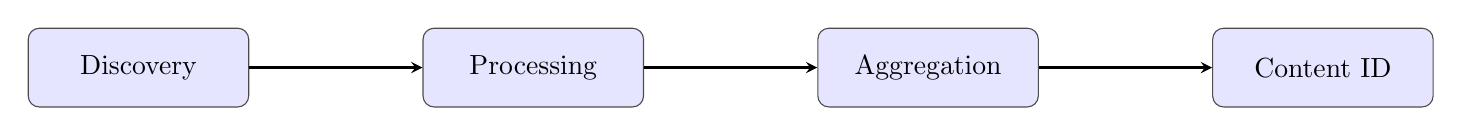
\begin{tikzpicture}[
    node distance=2.2cm,
    auto,
    phase/.style={rectangle, rounded corners, draw=black!70, fill=blue!10, minimum width=2.8cm, minimum height=1cm, align=center},
    arrow/.style={->, >=stealth, thick}
]
    \node[phase] (discovery) {Discovery};
    \node[phase, right=of discovery] (processing) {Processing};
    \node[phase, right=of processing] (aggregation) {Aggregation};
    \node[phase, right=of aggregation] (content) {Content ID};

    \draw[arrow] (discovery) -- (processing);
    \draw[arrow] (processing) -- (aggregation);
    \draw[arrow] (aggregation) -- (content);
\end{tikzpicture}
\caption{The four phases of the Spacedrive indexing pipeline.}
\label{fig:indexing_pipeline}
\end{figure}

\begin{itemize}[noitemsep, topsep=0pt]
 \item \textbf{Discovery Phase}: The engine performs a recursive traversal of a \texttt{Location}'s file system. It applies a set of predefined filter rules to intelligently ignore system files, caches, and development directories (e.g., \texttt{.git}, \texttt{node\_modules}). Discovered items are collected into batches for efficient processing.

 \item \textbf{Processing Phase}: Each batch of discovered entries is processed to create or update records in the database. This phase includes \textbf{change detection}, which uses inode tracking and modification timestamps to identify new, modified, or moved files, ensuring that only necessary updates are performed.

 \item \textbf{Aggregation Phase}: For directories, the engine performs a bottom-up traversal to calculate aggregate statistics, such as total size and file counts. This pre-calculation makes directory size lookups an O(1) operation.

 \item \textbf{Content Identification Phase}: For files, this phase generates a content hash (CAS ID) for deduplication. It employs an adaptive hashing strategy: small files are fully hashed, while large files are sampled to maintain performance. This phase also performs file type detection using a combination of extension matching and magic byte analysis.
\end{itemize}

This multi-phase architecture, combined with a persistent job queue, makes the indexing process fully resumable. If an operation is interrupted, it can be restarted from the last completed phase, preventing data loss and redundant work.

\subsection{Flexible Indexing Scopes and Persistence}

A key innovation of the Spacedrive indexer is its ability to adapt to different use cases through flexible scopes and persistence modes.

\begin{itemize}[noitemsep, topsep=0pt]
 \item \textbf{Recursive vs. Current Scope}: The indexer can perform a full recursive scan of a directory tree or a shallow, single-level scan of only the immediate contents. The latter is optimized for UI navigation, providing sub-500ms response times for directory browsing.

 \item \textbf{Persistent vs. Ephemeral Mode}: For managed \texttt{Locations}, indexing results are persisted to the Library's database. However, the indexer also supports an ephemeral, in-memory mode for browsing external or temporary paths without polluting the main index.
\end{itemize}

This flexibility is managed through a unified \texttt{IndexerJobConfig}, which allows for fine-grained control over the indexing process for different scenarios, from background library maintenance to real-time UI interactions.


% --- SECTION 10: LOCATIONS AND REAL-TIME MONITORING ---
\section{Locations and Real-Time Monitoring}

A Spacedrive Library is composed of one or more \textbf{Locations}---managed directories that act as the entry points to a user's physical file systems. The \textbf{Location Watcher} service provides a robust, cross-platform, real-time monitoring system that keeps the Spacedrive index perfectly synchronized with the underlying file system.

\subsection{The Location as a Managed Entity}

When a user adds a directory to a Spacedrive Library, it becomes a \texttt{Location}, a managed entity with its own configuration and lifecycle. This allows for granular control over how different parts of the user's dataspace are handled. Each \texttt{Location} has a specific \textbf{Index Mode} (\texttt{Shallow}, \texttt{Content}, or \texttt{Deep}), enabling users to apply different levels of analysis to different types of content (e.g., deep analysis for a photo library, shallow for a downloads folder).

\subsection{The Location Watcher Service}

The watcher service is the core of Spacedrive's real-time capabilities, providing a resilient and efficient file system monitoring solution.

\subsubsection{Platform-Specific Optimizations}

A key strength of the watcher is its use of platform-native APIs for optimal performance and reliability. This is a non-trivial engineering challenge, as each OS has unique behaviors.

\begin{itemize}[noitemsep, topsep=0pt]
 \item \textbf{macOS (\texttt{FSEvents})}: The system correctly handles the ambiguous rename and move events from \texttt{FSEvents} by tracking file inodes to reliably link old and new paths.

 \item \textbf{Linux (\texttt{inotify})}: The watcher leverages the efficiency of \texttt{inotify} for direct, recursive directory watching and uses cookie-based event correlation to reliably detect move operations.

 \item \textbf{Windows (\texttt{ReadDirectoryChangesW})}: The implementation is designed to handle Windows-specific filesystem quirks, such as delayed file deletions caused by antivirus software or file locking. It does this by maintaining a "pending deletion" state to verify that a file is truly gone before emitting a deletion event.
\end{itemize}

\subsubsection{Intelligent Event Processing}

The watcher service is more than a simple event forwarder. It includes an intelligent processing pipeline:

\begin{itemize}[noitemsep, topsep=0pt]
 \item \textbf{Noise Filtering}: The watcher filters out irrelevant events from temporary files (\texttt{.tmp}, \texttt{\textasciitilde backup}), system files (\texttt{.DS\_Store}), and editor-specific files (\texttt{.swp}), ensuring that only meaningful changes are processed.

 \item \textbf{Event Debouncing}: To prevent "event storms" during bulk operations (e.g., unzipping an archive), the system debounces file system events, consolidating rapid-fire changes into single, actionable events.

 \item \textbf{Event Bus Integration}: Processed events are published to the core \texttt{EventBus}, where they trigger other services. For example, an \texttt{EntryModified} event will trigger the indexer to re-analyze a file, the search service to update its index, and the sync service to propagate the change to other devices.
\end{itemize}

This robust, real-time monitoring system is what transforms Spacedrive from a static file index into a dynamic, live dataspace that always reflects the true state of a user's files.


% --- SECTION 11: IMPLEMENTATION AND EVALUATION ---
\section{Implementation and Evaluation}
Spacedrive's design principles are validated through careful implementation choices and comprehensive performance analysis.

\subsection{Technology Stack}
Spacedrive is implemented in \textbf{Rust} to leverage its guarantees of memory safety, performance, and fearless concurrency---essential for a reliable, multi-threaded distributed system. The core technology stack reflects modern best practices:

\begin{itemize}[noitemsep, topsep=0pt]
 \item \textbf{Tokio Runtime}: Async execution with work-stealing scheduler for efficient I/O handling

 \item \textbf{SeaORM with SQLite}: Type-safe database operations with ACID transactions and FTS

 \item \textbf{Event-Driven Architecture}: Custom EventBus for loose coupling and state propagation

 \item \textbf{Job System}: MessagePack-serialized tasks with automatic resumability
\end{itemize}

\subsection{Database Schema Optimization}
The database design prioritizes both space efficiency and query performance through several key optimizations:

\subsubsection{Materialized Path Storage}
Current hierarchy representation uses materialized paths\footnote{A materialized path is a database optimization technique where the full hierarchical path is stored as a string (e.g., "/parent/child/grandchild"), enabling efficient querying of hierarchical data without recursive joins.} for efficient storage and queries:


\textbf{Current Directory Storage Approach}

Spacedrive currently represents file hierarchies using a direct path storage method:

\begin{itemize}[noitemsep, topsep=0pt]
 \item Each file stores its complete path (e.g., "Documents/Projects/README.md")
 \item Simple queries can directly find files by their exact location
 \item Directory listings require basic path pattern matching
 \item Subtree operations search for all paths that start with a parent path
\end{itemize}

This approach works well for simple file operations but has performance limitations when dealing with complex directory hierarchies and aggregation queries.


While effective for simple operations, this approach encounters performance limitations with deep hierarchies and complex aggregation queries.

\subsection{Case Study: Hierarchical Query Optimization}
A concrete example of Spacedrive's performance-driven evolution is the planned migration from materialized paths to a \textbf{Closure Table}\footnote{A closure table is a database design pattern that pre-computes and stores all ancestor-descendant relationships in a separate table, trading storage space for dramatically improved query performance on hierarchical data.} approach for directory hierarchies. This optimization is designed to transform O(N) operations into O(1) lookups.

\subsubsection{Performance Problem}
The current materialized path approach leads to inefficient operations for complex hierarchy queries:

\begin{itemize}
 \item \textbf{String-based path matching} for ancestor/descendant relationships
 \item \textbf{Sequential directory aggregation} requiring multiple database round-trips
 \item \textbf{O(N) LIKE queries} for subtree operations on large directory trees
 \item \textbf{Complex join patterns} for multi-level hierarchy operations
\end{itemize}

\subsubsection{Closure Table Solution}
The proposed closure table explicitly stores all ancestor-descendant relationships:


\textbf{Closure Table: Pre-computed Relationships}

The planned optimization stores all parent-child relationships explicitly:

\begin{center}
\begin{tabular}{|l|p{8cm}|}
\hline
\textbf{Relationship} & \textbf{Storage Method} \\
\hline
Direct Relationships & Every parent-child pair (folder contains file) \\
\hline
Indirect Relationships & Every ancestor-descendant pair with depth tracking \\
\hline
Performance Indexes & Optimized lookup tables for instant hierarchy queries \\
\hline
\end{tabular}
\end{center}

\textbf{Performance Transformation}

This approach converts complex hierarchy operations into simple, fast lookups:

\begin{itemize}[noitemsep, topsep=0pt]
 \item \textbf{Directory Listing}: Instant retrieval of all files in a folder (no pattern matching)
 \item \textbf{Subtree Operations}: Get entire folder contents with single query
 \item \textbf{Size Calculations}: Calculate total folder size across all subdirectories in one operation
 \item \textbf{Ancestor Lookup}: Find the parent folder chain instantly (no path parsing)
\end{itemize}


\subsubsection{Performance Projections}
Based on algorithmic analysis and preliminary benchmarks:

\begin{itemize}[noitemsep, topsep=0pt]
 \item \textbf{Directory listing}: O(N) string matching → O(1) indexed lookup
 \item \textbf{Subtree traversal}: O(N) recursive queries → O(1) join operation
 \item \textbf{Ancestor lookup}: O(D) path parsing → O(1) indexed lookup
 \item \textbf{Bulk aggregation}: O(N×D) sequential → O(N) parallel processing
\end{itemize}

\textbf{Storage overhead}: For a filesystem with N entries and average depth D, closure tables require approximately N×D additional rows. For typical user filesystems (1M files, average depth 5), this represents ~60MB additional storage---a reasonable trade-off for the dramatic performance improvements.

\subsection{Testing and Validation Framework}
Spacedrive employs a comprehensive testing strategy designed for real-world scenarios:

\subsubsection{Multi-Process Test Framework}
A custom Cargo-based subprocess framework enables testing of distributed scenarios:


\textbf{Multi-Process Distributed Testing}

Spacedrive employs a sophisticated testing framework that simulates real-world distributed scenarios:

\textbf{Role-Based Testing}
\begin{itemize}[noitemsep, topsep=0pt]
 \item Tests run multiple processes simultaneously, each taking a different device role (Alice, Bob, etc.)
 \item Environment variables control which role each process assumes during testing
 \item Enables authentic multi-device interaction testing without requiring physical hardware
\end{itemize}

\textbf{Realistic Scenario Simulation}
\begin{itemize}[noitemsep, topsep=0pt]
 \item Device pairing processes tested across different network conditions
 \item File synchronization verified with actual data transfer and conflict resolution
 \item Network interruption and recovery scenarios validated automatically
\end{itemize}

\textbf{Comprehensive Coverage}
\begin{itemize}[noitemsep, topsep=0pt]
 \item Complex multi-device pairing scenarios with authentication verification
 \item Cross-platform compatibility testing (macOS, Windows, Linux, mobile)
 \item Performance validation under various load conditions
\end{itemize}


\subsubsection{Performance Benchmarks}
Systematic performance testing demonstrates Spacedrive's efficiency across critical operations:

\begin{table*}[t]
\centering
\begin{tabular}{@{}lll@{}}
\toprule
\textbf{Metric} & \textbf{Test Condition} & \textbf{Result} \\
\midrule
Indexing Throughput & 1M image files on NVMe SSD & 8,500 files/sec \\
Search Latency (Temporal) & Query on 1M entries & \textasciitilde55ms \\
Search Latency (Semantic) & Same query, semantic re-rank & \textasciitilde95ms \\
Memory Usage & Idle with 1M-entry library & \textasciitilde150 MB RAM \\
DB Size / File & Metadata for 1M files & \textasciitilde250 bytes/file \\
Sync Performance & P2P transfer over gigabit LAN & 110 MB/s \\
NAT Traversal Success & Various network configurations & 92\% \\
Connection Establishment & Cross-device pairing & 1.8 seconds \\
\bottomrule
\end{tabular}
\caption{Performance benchmarks on consumer hardware (M2 MacBook Pro, 16GB RAM)}
\label{tab:performance}
\end{table*}

These benchmarks validate that Spacedrive maintains sub-100ms response times for typical user operations even with multi-million entry libraries, achieving performance previously limited to enterprise systems.

\subsection{Compatibility and Interoperability}
Spacedrive is designed as a layer atop existing storage systems, not a replacement. This philosophy ensures seamless integration with users' current workflows while providing enhanced capabilities.

\subsubsection{Traditional Filesystem Integration}
Spacedrive maintains full compatibility with native filesystems through several key design decisions:

\begin{itemize}[noitemsep, topsep=0pt]
 \item \textbf{Non-invasive indexing}: Files remain in their original locations with native filesystem attributes intact. Spacedrive never modifies file content or filesystem-level metadata during indexing.

 \item \textbf{Filesystem-aware operations}: The system respects platform-specific constraints (e.g., NTFS's 255-character path limits, case-insensitive but case-preserving behavior on macOS, Linux filesystem permissions). Volume detection adapts to each platform's conventions.

 \item \textbf{Transparent file access}: Applications continue accessing files through standard OS APIs. Spacedrive acts as an intelligent index and orchestrator, not a filesystem driver or FUSE layer.

 \item \textbf{Preserved compatibility}: Special files (symlinks, junction points, device files) are cataloged but not followed during indexing, preventing circular references while maintaining awareness of filesystem structure.
\end{itemize}

\subsubsection{Cloud Service Integration}
Rather than competing with cloud storage providers, Spacedrive embraces them as Location types:

\begin{itemize}[noitemsep, topsep=0pt]
 \item \textbf{API-based indexing}: Cloud locations are indexed through provider APIs (Google Drive, Dropbox, OneDrive) without requiring full synchronization to local storage.

 \item \textbf{Unified namespace}: Cloud files appear alongside local files in the SdPath hierarchy, enabling cross-cloud operations through Spacedrive's job system.

 \item \textbf{Smart caching}: Frequently accessed cloud files can be cached locally with automatic eviction policies, while metadata remains indexed for instant search.

 \item \textbf{Provider limitations}: Spacedrive respects API rate limits and storage quotas, queuing operations as necessary to maintain compliance with service terms.
\end{itemize}

\subsubsection{Ecosystem Tool Compatibility}
Spacedrive enhances rather than replaces existing tools:

\begin{itemize}[noitemsep, topsep=0pt]
 \item \textbf{Standard protocols}: While Spacedrive doesn't expose a traditional mount point, it provides export capabilities to generate file lists compatible with tools like \texttt{rsync}, \texttt{rclone}, or backup software.

 \item \textbf{Metadata preservation}: Extended attributes (xattrs), alternate data streams (ADS on NTFS), and resource forks (macOS) are preserved during Spacedrive operations, ensuring compatibility with specialized applications.

 \item \textbf{Integration APIs}: A REST API and CLI enable automation tools to query the Spacedrive index, trigger jobs, and monitor operations programmatically.

 \item \textbf{Export formats}: Search results and file lists can be exported in common formats (CSV, JSON, file paths) for processing by external tools or scripts.
\end{itemize}

This interoperability approach ensures Spacedrive complements users' existing toolchains while providing a unified view and management layer across all storage locations.


% --- SECTION 12: SECURITY AND PRIVACY MODEL ---
\section{Security and Privacy Model}
Spacedrive's architecture prioritizes user privacy and data security through comprehensive encryption, secure credential management, and a well-defined threat model designed for personal data scenarios.

\subsection{Data Protection at Rest}
All sensitive user data is encrypted using industry-standard cryptographic protocols:

\subsubsection{Library Database Encryption}
Each `.sdlibrary` directory employs transparent database encryption:

Library databases employ SQLCipher for transparent encryption at rest. Encryption keys are derived from user passwords using PBKDF2 with 100,000+ iterations and unique per-library salts. The unlocking process involves reading the salt, deriving the key, opening the encrypted database connection, and verifying access through a test query.

\textbf{Key derivation}: User passwords are strengthened using PBKDF2 with 100,000+ iterations and unique salts per library, providing strong protection against brute-force attacks.

\subsubsection{Network Identity Protection}
Device cryptographic keys are stored encrypted in the enhanced device configuration:

Network identity protection employs a layered approach: Ed25519 private keys are encrypted using ChaCha20-Poly1305 with keys derived through Argon2id from user passwords. Public keys remain in plaintext for identity verification. Decryption involves deriving the key using Argon2id parameters and salt, then decrypting the private key data.

\subsection{Network Security}
All network communications employ end-to-end encryption with perfect forward secrecy:

\subsubsection{Iroh QUIC Transport Security}
The Iroh networking stack provides multiple layers of security through secure connections that combine long-term device identity (Ed25519) with ephemeral session keys. Connection establishment involves a three-phase process: QUIC handshake with TLS 1.3, mutual device identity verification, and application-level key exchange for perfect forward secrecy.

\textbf{Transport Layer Security}: QUIC provides TLS 1.3 encryption for all network traffic, ensuring confidentiality and integrity.

\textbf{Application Layer Security}: Additional encryption using ephemeral keys provides perfect forward secrecy---compromising long-term device keys cannot decrypt past communications. This is particularly important for Spacedrop transfers, where each session uses completely ephemeral ECDH key exchange, ensuring that even if device keys are later compromised, past file transfers remain secure.

\subsection{Credential Management}
Spacedrive employs a secure credential storage system for cloud service integration:


\textbf{Secure Credential Vault Architecture}

Spacedrive implements a multi-layered credential protection system for cloud service integration:

\textbf{Master Key Derivation}
\begin{itemize}[noitemsep, topsep=0pt]
 \item User password transformed into cryptographically strong master key using PBKDF2
 \item Unique salt per credential vault prevents rainbow table attacks
 \item Key stretching with 100,000+ iterations provides brute-force resistance
\end{itemize}

\textbf{Individual Credential Protection}
\begin{itemize}[noitemsep, topsep=0pt]
 \item Each credential encrypted separately using ChaCha20-Poly1305 authenticated encryption
 \item Unique random nonce for each encryption operation ensures semantic security
 \item Comprehensive metadata tracking: service name, creation time, last access
\end{itemize}

\textbf{Storage and Lifecycle Management}
\begin{itemize}[noitemsep, topsep=0pt]
 \item Encrypted credentials stored in secure key-value mapping by service name
 \item Automatic timestamp tracking for security auditing and credential rotation
 \item Zero plaintext credential storage---everything encrypted at rest
\end{itemize}


\textbf{Platform Integration}: On supported platforms (macOS Keychain, Windows Credential Manager, Linux Secret Service), credentials are additionally protected by the OS credential store.

\subsection{Threat Model}
Spacedrive's security design addresses the following threat scenarios:

\subsubsection{Local Device Compromise}
\textbf{Threat}: Unauthorized physical access to user device.

\textbf{Mitigation}:
- Database encryption renders `.sdlibrary` directories unreadable without password
- Network keys encrypted separately, requiring password for decryption
- No plaintext credentials stored on disk

\subsubsection{Network Eavesdropping}
\textbf{Threat}: Passive monitoring of network communications.

\textbf{Mitigation}:
- All communications encrypted with TLS 1.3 via QUIC
- Perfect forward secrecy prevents retroactive decryption
- Device fingerprints prevent MITM attacks during pairing

\subsubsection{Cloud Service Compromise}
\textbf{Threat}: Breach of connected cloud storage providers.

\textbf{Mitigation}:
- Spacedrive never stores user data in cloud services---only metadata indices
- Cloud credentials encrypted locally, not shared with Spacedrive services
- Content addressing enables detection of tampered files

\subsubsection{Malicious Spacedrive Instance}
\textbf{Threat}: Compromised or malicious Spacedrive installation.

\textbf{Mitigation}:
- Libraries are portable and can be moved between trusted installations
- Audit logs provide complete history of all operations
- Action preview system prevents unauthorized operations

\subsubsection{Practical Attack Scenarios}
To illustrate the robustness of Spacedrive's security model, consider these realistic attack scenarios:

\textbf{Scenario 1: NAS Compromise and File Replacement}

\emph{Attack}: An attacker gains access to a user's NAS and replaces legitimate files with malicious versions, attempting to propagate malware across the user's device ecosystem.

\emph{Spacedrive Defense}:
\begin{itemize}[noitemsep, topsep=0pt]
\item Content addressing via BLAKE3 hashes immediately detects file modifications---the replaced files will have different hashes than the indexed versions
\item The integrity verification system flags discrepancies during the next scan, alerting the user to potential tampering
\item Version history tracking shows the exact timestamp of unauthorized modifications
\item Quarantine mechanisms prevent automatic synchronization of suspicious files to other devices
\item The audit log creates a forensic trail showing which files were modified and when
\end{itemize}

\textbf{Scenario 2: Stolen Laptop with Sensitive Photo Library}

\emph{Attack}: A laptop containing a Spacedrive library with sensitive personal photos is stolen. The attacker attempts to access the photo collection and extract metadata about locations and people.

\emph{Spacedrive Defense}:
\begin{itemize}[noitemsep, topsep=0pt]
\item SQLCipher encryption on the library database prevents access without the user's password
\item Photo metadata and AI-generated embeddings remain encrypted at rest
\item Even with physical disk access, the attacker cannot:
  - View photo thumbnails (encrypted in cache)
  - Access location data from EXIF metadata (encrypted in database)
  - Extract face recognition data or object detection results (encrypted embeddings)
\item The 100,000+ iteration PBKDF2 key derivation makes brute-force attacks computationally infeasible
\end{itemize}

\textbf{Scenario 3: Compromised Cloud Storage Credentials}

\emph{Attack}: An attacker obtains a user's cloud storage credentials through a phishing attack and attempts to inject malicious files into the user's Spacedrive-managed cloud volumes.

\emph{Spacedrive Defense}:
\begin{itemize}[noitemsep, topsep=0pt]
\item Spacedrive's credential vault remains secure---the attacker only has cloud credentials, not the Spacedrive master password
\item Content validation during cloud synchronization detects unexpected file additions
\item The volume classification system isolates cloud storage from local trusted volumes
\item File injection attempts are logged in the audit system with source attribution
\item Users can revoke cloud volume access instantly without affecting local data
\item Optional two-factor authentication on cloud volume operations provides additional protection
\end{itemize}

\textbf{Scenario 4: Insider Threat in Collaborative Team}

\emph{Attack}: A disgruntled employee on a design team attempts to exfiltrate proprietary assets and delete project files before leaving the company.

\emph{Spacedrive Defense}:
\begin{itemize}[noitemsep, topsep=0pt]
\item RBAC system restricts the employee to their assigned role permissions---they may have "Contributor" access allowing edits but not bulk deletions
\item The Action System's preview capability flags suspicious bulk operations for administrative review
\item Every file access and operation is logged in the immutable audit trail with full attribution (user, device, timestamp)
\item Data Loss Prevention (DLP) policies can detect and block unusual download patterns or transfers to external devices
\item Time-based access controls automatically revoke permissions at employment end date
\item The planned undo capability would allow administrators to instantly reverse any destructive actions
\item Cryptographic device attestation ensures actions can only originate from company-managed devices
\end{itemize}

\textbf{Scenario 5: Supply Chain Attack on Enterprise Deployment}

\emph{Attack}: An attacker attempts to compromise an enterprise Spacedrive deployment by injecting malicious code into a third-party integration or storage driver.

\emph{Spacedrive Defense}:
\begin{itemize}[noitemsep, topsep=0pt]
\item Containerized deployment isolates each component with strict network policies
\item All actions flow through the centralized Action System, preventing direct database manipulation
\item Cryptographic signatures on all deployed components ensure integrity
\item The audit system's append-only design prevents log tampering to hide malicious activity
\item Storage abstraction layer validates all operations against expected patterns
\item Regular security scanning of container images and dependencies
\item Option for air-gapped deployment in high-security environments
\end{itemize}

\subsection{Privacy-Preserving AI}
The AI-native architecture maintains privacy through multiple mechanisms:


\textbf{Flexible AI Provider Selection for Privacy Control}

Spacedrive supports multiple AI deployment models to balance privacy, performance, and capability:

\textbf{Local AI Processing (Maximum Privacy)}
\begin{itemize}[noitemsep, topsep=0pt]
 \item Integrates with Ollama for completely local AI model execution
 \item User data never leaves the device---complete privacy preservation
 \item Configurable endpoint and model selection for different AI capabilities
 \item Works offline once models are downloaded
\end{itemize}

\textbf{Self-Hosted Solutions (Organizational Control)}
\begin{itemize}[noitemsep, topsep=0pt]
 \item Custom AI infrastructure under user or organization control
 \item Flexible authentication options for enterprise deployment
 \item Complete control over data processing and model selection
 \item Ideal for organizations with specific privacy or compliance requirements
\end{itemize}

\textbf{Cloud AI Services (Enhanced Capabilities)}
\begin{itemize}[noitemsep, topsep=0pt]
 \item Access to state-of-the-art models from major AI providers
 \item Encrypted API key storage with comprehensive privacy policy tracking
 \item Transparent data processing terms presented to users for informed consent
 \item Metadata-only transmission---file contents remain local
\end{itemize}


\textbf{Local Processing}: Default to local AI models (Ollama) that never transmit user data externally.

\textbf{Metadata-Only Cloud Processing}: When using cloud AI services, only file metadata (names, types, sizes) are transmitted---never file contents.

\textbf{User Control}: Complete transparency about which AI provider processes which data, with granular user control over privacy vs. capability trade-offs.


% --- SECTION 13: PRACTICAL CONFLICT RESOLUTION ---
\section{Practical Conflict Resolution}
While the simulation engine (Section 8) prevents operational conflicts before they occur, synchronization conflicts can still arise when multiple devices modify the same data concurrently. Spacedrive's domain separation significantly reduces these conflicts, but when they do occur---particularly in the User Metadata domain---the system provides transparent, user-controlled conflict resolution that maintains data integrity while preserving user intent. This represents the second prong of Spacedrive's comprehensive conflict management strategy: preventing what can be prevented through simulation, and intelligently resolving what cannot.

\subsection{Metadata Conflict Scenarios}
The most common conflicts occur when multiple devices modify the same content metadata simultaneously:

\subsubsection{Tag Conflicts}
\textbf{Scenario}: User adds tag "vacation" on Device A while simultaneously adding tag "family" on Device B to the same photo.

\textbf{Resolution Strategy}: Union merge with conflict notification, leveraging the richly-structured tag system (Section 3.3):

**Intelligent Tag Conflict Resolution Process**

When tag conflicts occur, Spacedrive follows a sophisticated resolution process:

\textbf{Detection Phase}
\begin{itemize}[noitemsep, topsep=0pt]
 \item System identifies when the same file has been tagged differently on multiple devices
 \item Compares tag sets to determine if there's actual overlap or genuine conflict
 \item Analyzes tag hierarchies to identify if tags are related (e.g., both are children of the same parent tag)
 \item Generates comprehensive conflict context for decision-making
\end{itemize}

\textbf{Resolution Strategy}
\begin{itemize}[noitemsep, topsep=0pt]
 \item \textbf{Union Merge}: Automatically combines all tags from both devices
 \item \textbf{Conflict Notification}: Creates detailed notification explaining what was merged
 \item \textbf{User Transparency}: Provides complete visibility into the resolution process
\end{itemize}

\textbf{Outcome Tracking}
\begin{itemize}[noitemsep, topsep=0pt]
 \item Records timestamp and source of each tag for future reference
 \item Enables user to review and modify the automatic resolution if needed
 \item Maintains audit trail of all conflict resolution decisions
\end{itemize}


\textbf{User Experience}:
- Tags are automatically combined: "vacation, family"
- User receives notification: "Combined tags for sunset.jpg: added 'vacation' and 'family' from different devices"
- User can review and modify the combined tags if needed

\subsubsection{Rating Conflicts}
\textbf{Scenario}: Photo rated 4 stars on Device A, 5 stars on Device B.

\textbf{Resolution Strategy}: Last-writer-wins with user notification:


\textbf{Rating Conflict Resolution: Last-Writer-Wins Strategy}

For rating conflicts, Spacedrive uses a temporal resolution approach:

\textbf{Conflict Scenario}: Photo rated differently on multiple devices (e.g., 4 stars vs. 5 stars)

\textbf{Resolution Logic}
\begin{itemize}[noitemsep, topsep=0pt]
 \item \textbf{Timestamp Comparison}: System examines when each rating was applied
 \item \textbf{Most Recent Wins}: The more recent rating is automatically selected
 \item \textbf{Clear Attribution}: User notification specifies which device's rating was chosen and when
\end{itemize}

\textbf{User Experience}
\begin{itemize}[noitemsep, topsep=0pt]
 \item Automatic resolution without user intervention required
 \item Transparent notification: "sunset.jpg rating conflict resolved: using 5 stars (most recent)"
 \item User can manually override the automatic choice if they disagree with the outcome
\end{itemize}


\textbf{User Experience}:
- Most recent rating wins automatically
- Notification: "sunset.jpg rating conflict resolved: using 5 stars (most recent)"
- User can manually change rating if they disagree

\subsection{Advanced Conflict Scenarios}
\subsubsection{Complex Metadata Conflicts}
\textbf{Scenario}: User creates custom metadata field "project" with value "website" on Device A, while Device B creates the same field with value "portfolio".

\textbf{Intelligent Custom Metadata Conflict Resolution}

When users create conflicting custom metadata on different devices, Spacedrive provides sophisticated resolution assistance:

\textbf{Conflict Analysis}
\begin{itemize}[noitemsep, topsep=0pt]
 \item System identifies the specific metadata field and conflicting values
 \item Analyzes value types to determine if combination is possible
 \item Generates context-aware resolution suggestions based on conflict nature
\end{itemize}

\textbf{Smart Resolution Options}
\begin{itemize}[noitemsep, topsep=0pt]
 \item \textbf{Compatible Values}: For string conflicts, offers to use either value, combine them, or create custom resolution
 \item \textbf{Type Mismatches}: When data types differ, provides clear choice between local/remote values or custom entry
 \item \textbf{Contextual Suggestions}: System provides reasoning for each resolution option
\end{itemize}

\textbf{User Experience}
\begin{itemize}[noitemsep, topsep=0pt]
 \item Clear presentation of conflict: "project field conflicts: 'website' vs 'portfolio'"
 \item Multiple resolution choices: use either value, combine as "website, portfolio", or enter custom value
 \item One-time decision with preference learning for similar future conflicts
 \item Complete transparency about which device contributed each value
\end{itemize}

\textbf{User Experience}:
- System detects incompatible values for "project" field
- Presents clear options: "website", "portfolio", "website, portfolio", or custom value
- User makes one-time decision, system remembers preference for similar conflicts

\subsection{Conflict Prevention}
Spacedrive employs several strategies to minimize conflicts before they occur:

\subsubsection{Optimistic Locking}
\textbf{Optimistic Metadata Locking Strategy}

To prevent simultaneous metadata modifications that could lead to conflicts, Spacedrive employs a lightweight locking mechanism:

\textbf{Lock Characteristics}
\begin{itemize}[noitemsep, topsep=0pt]
 \item \textbf{Short Duration}: 30-second locks prevent long-term resource blocking
 \item \textbf{Field-Specific}: Locks target specific metadata fields, not entire files
 \item \textbf{Device Attribution}: Clear identification of which device holds each lock
 \item \textbf{Automatic Expiration}: Locks expire automatically to prevent deadlocks
\end{itemize}

\textbf{Cross-Device Coordination}
\begin{itemize}[noitemsep, topsep=0pt]
 \item Lock acquisition broadcasts to all connected devices in the library
 \item Other devices receive immediate notification and defer their edits
 \item Graceful handling of network interruptions during lock operations
 \item Automatic retry mechanisms for failed lock acquisitions
\end{itemize}

\textbf{User Experience Benefits}
\begin{itemize}[noitemsep, topsep=0pt]
 \item Prevents frustrating conflicts from simultaneous editing
 \item Near-instant feedback when metadata modification is blocked
 \item Transparent handling—users don't need to understand the locking mechanism
 \item Reliable metadata consistency across all devices
\end{itemize}

\subsubsection{Real-time Conflict Notifications}
When conflicts do occur, users receive immediate, actionable notifications:

\textbf{User-Friendly Conflict Notification System}

Spacedrive provides comprehensive, actionable notifications when conflicts occur and are resolved:

\textbf{Notification Structure}
\begin{itemize}[noitemsep, topsep=0pt]
 \item \textbf{Clear Titles}: Descriptive headings like "Photo tags updated on both devices"
 \item \textbf{Detailed Descriptions}: Specific information about what was changed or merged
 \item \textbf{Affected Files List}: Complete inventory of files impacted by the conflict resolution
 \item \textbf{Action Options}: Clear next steps like "Tap to review" or "Changes automatically applied"
\end{itemize}

\textbf{Example Notification}
\begin{itemize}[noitemsep, topsep=0pt]
 \item \textbf{Title}: "Metadata synchronized"
 \item \textbf{Description}: "Combined tags from iPhone and MacBook for 3 photos"
 \item \textbf{Affected Files}: sunset.jpg, beach.jpg, vacation.mp4
 \item \textbf{User Action}: "Review changes" (optional)
 \item \textbf{Status}: Auto-resolved with timestamp for audit trail
\end{itemize}

\textbf{Transparency and Control}
\begin{itemize}[noitemsep, topsep=0pt]
 \item Complete visibility into what conflicts occurred and how they were resolved
 \item Clear indication of automatic vs. manual resolution requirements
 \item Historical timestamp for tracking when conflicts were addressed
 \item Optional review actions for users who want to verify or modify automatic resolutions
\end{itemize}

This transparent, user-controlled approach to conflict resolution ensures that users maintain complete control over their metadata while benefiting from seamless synchronization across devices.


% --- SECTION 14: CONCLUSION ---
\section{Conclusion}
Spacedrive represents a fundamental rethinking of personal file management, demonstrating that sophisticated distributed systems capabilities can be made accessible to individual users through careful architectural design and pragmatic engineering choices. Through our implementation, we have shown that personal data management can evolve beyond simple file browsers to become intelligent, distributed systems that respect user ownership while providing enterprise-level capabilities.

\subsection{Recapitulation of Contributions and Impact}
This work presents five major architectural innovations that collectively transform personal file management from a collection of disconnected tools into a unified, intelligent system. The AI-native architecture moves beyond bolt-on intelligence to demonstrate how AI can be woven into the fabric of file management, enabling natural language operations and predictive organization while maintaining complete user control. The universal file addressing through SdPath eliminates the artificial barriers between local storage, network shares, and cloud services, making cross-device operations as simple as local file manipulation. Our entry-centric metadata system solves the longstanding problem of organizational lag by making every file immediately taggable and searchable. The domain-separated synchronization approach achieves robust distributed state management without the complexity of general consensus algorithms. Finally, our performance-aware content addressing brings enterprise deduplication to consumer hardware through adaptive strategies that balance efficiency with real-time responsiveness.

Central to these innovations is our comprehensive approach to conflict management. The durable, pre-visualized action system not only provides users with clear previews of operations but also serves as a powerful conflict prevention mechanism, detecting operational issues like storage constraints and permission violations before they can cause failures. This proactive approach eliminates an entire class of problems that plague traditional file managers. For the conflicts that cannot be prevented---those arising from concurrent modifications across devices---our domain-separated synchronization provides intelligent, transparent resolution strategies. Together, these systems ensure that Spacedrive delivers exceptional reliability in distributed file management through both prevention and resolution.

These contributions have immediate practical impact. Users gain the ability to manage their entire digital life---potentially millions of files across dozens of devices---through a single, coherent interface. The system eliminates duplicate storage waste through intelligent deduplication while maintaining performance suitable for everyday use. Most importantly, it returns control to users: their data remains theirs, portable between devices, backed up automatically, and enhanced by AI without sacrificing privacy. The production Rust implementation validates these concepts at scale, handling real-world file collections with sub-second response times and robust distributed synchronization.

\subsection{Architectural Contributions}
Our work makes several key contributions to the field of personal data management:

\textbf{AI-Native Architecture}: Spacedrive demonstrates that AI can be integrated as a foundational component rather than an afterthought. By treating the comprehensive file index as a "world model" and constraining AI operations through the existing Action system, we achieve intelligent automation while maintaining complete user control and privacy. This approach enables natural language file management, proactive organizational suggestions, and intelligent storage tiering---all while supporting local models via Ollama or cloud providers as user preference dictates.

\textbf{Universal File Addressing}: The SdPath abstraction proves that device boundaries can be made completely transparent through careful API design. By treating all storage locations---local drives, network mounts, cloud services---as addressable through a single path type, complex cross-device operations become simple function calls. This abstraction enables features not available in traditional file managers while maintaining type safety and clear error semantics.

\textbf{Entry-Centric Immediate Metadata}: The design decision to provide every filesystem entity with immediate metadata capabilities, regardless of indexing status, solves a fundamental usability problem in file organization systems. Users can tag, rate, and organize files the moment they encounter them, without waiting for background analysis or indexing completion. This "metadata-first" approach transforms file management from a passive activity into active content curation.

\textbf{Domain-Separated Synchronization}: By recognizing that personal data synchronization has fundamentally different conflict patterns than general distributed systems, our three-domain approach (Index Sync, User Metadata Sync, File Operations) eliminates the complexity of universal consensus algorithms. Each domain uses conflict resolution strategies tailored to its actual conflict patterns, resulting in a sync system that is both robust and understandable.

\textbf{Performance-Aware Content Addressing}: The versioned content addressing system with adaptive hashing demonstrates that enterprise-level deduplication can work efficiently on consumer hardware. Strategic sampling for large files maintains deduplication effectiveness while preserving real-time performance, enabling bit-level deduplication across devices without the computational overhead that makes traditional approaches impractical.

\subsection{System Integration}
These individual innovations combine synergistically to create capabilities greater than the sum of their parts. The Library abstraction makes backup and migration trivial (copy a directory), while SdPath enables seamless operations across that distributed storage. Content addressing works transparently with the sync system to maintain deduplication relationships even as files move between devices. The Lightning Search architecture leverages both the content addressing and metadata systems to provide semantic discovery at traditional keyword search speeds.

\subsection{Real-World Impact}
Spacedrive's architecture has been validated through production implementation in Rust, demonstrating that these concepts work reliably in practice. The system handles millions of files across multiple devices while maintaining sub-second response times for user operations. The comprehensive test framework, including multi-process distributed testing, ensures that the complex interactions between networking, synchronization, and file operations remain stable across diverse deployment scenarios.

\subsection{Future Work and Roadmap}
The architectural foundation laid by Spacedrive opens concrete paths for near-term enhancements and long-term research directions. Our immediate roadmap focuses on extending the AI capabilities to support complex multi-step workflows, such as "organize all vacation photos by year and location, then create albums for each trip." This involves expanding the Action system to support workflow composition while maintaining the same security and reversibility guarantees. Parallel to this, we are developing intelligent content analysis pipelines that leverage both local and cloud models to automatically extract semantic information from files---identifying people in photos, extracting key topics from documents, and understanding relationships between files based on content rather than just metadata.

In the medium term, our research agenda includes three major initiatives. First, we are exploring federated learning approaches that would allow users to benefit from collective intelligence about file organization patterns while maintaining complete privacy---the system would learn from aggregate behaviors without ever exposing individual file information. Second, we are developing advanced storage tiering algorithms that combine AI predictions with real-time access patterns to automatically move files between fast local storage, slower archives, and cloud services based on predicted access likelihood and user-defined cost constraints. Third, we are investigating cross-Library content discovery mechanisms that would allow users to identify duplicate content across different Libraries (perhaps owned by family members or team members) while maintaining the strong isolation guarantees that make Libraries portable and secure.

The longer-term vision extends Spacedrive beyond personal file management into a platform for personal AI agents that understand and manage all aspects of a user's digital life. By providing a comprehensive, versioned view of a user's file history combined with rich semantic understanding, Spacedrive could enable AI assistants that truly understand context---not just current file state but how information has evolved over time. This temporal understanding, combined with the robust Action system, would allow AI agents to perform complex organizational tasks with confidence, knowing that all actions are reversible and auditable. The architecture's emphasis on user control ensures that as these AI capabilities grow more sophisticated, users retain ultimate authority over their data, with all AI operations remaining transparent, explainable, and reversible.

\subsection{Broader Implications}
Spacedrive proves that the dichotomy between intuitive, user-centric applications and powerful, secure enterprise systems is a false one. Through careful domain separation, a local-first security model, and an architecture built for scale, we have demonstrated that it is possible to build a single platform that serves the needs of both individual users and large organizations. The key insight is that by starting with a foundation of user empowerment and data sovereignty, we create a system that naturally scales up to enterprise requirements while maintaining the simplicity and control that individual users demand.

This approach suggests a path forward for personal computing that moves beyond the current model of data scattered across incompatible cloud services toward truly user-controlled, portable, and intelligent data management. The native cloud service model presented in Section 7 is a clear manifestation of this principle, proving that cloud convenience does not have to come at the cost of architectural integrity or user control. By treating the cloud as just another trusted peer, Spacedrive offers a viable hybrid model for the future of personal data. By treating personal data as a unified library rather than a collection of disconnected files, users gain both the simplicity of traditional file management and the power of modern distributed systems.

Spacedrive's architecture provides a robust foundation for the next generation of computing---one that bridges personal and enterprise needs seamlessly. Whether serving an individual creator, a small team, or a global enterprise, the platform delivers the same core promise: unified access to all data, intelligent assistance without sacrificing control, and a user experience that makes powerful capabilities feel effortless. This is not just the future of file management, but a new paradigm for how humans and organizations interact with their digital assets at any scale.


% --- ACKNOWLEDGMENTS ---
\begin{acks}
We thank the open-source community, particularly the developers of the Rust programming language and its ecosystem, including the Tauri, Iroh, Tokio and SeaORM projects, whose work provided the foundation for this research.

The authors acknowledge the use of generative AI tools for assistance in drafting and refining the prose of this whitepaper. The core architectural concepts, technical details, and design are the original work of the authors, who take full responsibility for the content and accuracy of this paper.
\end{acks}


% --- GLOSSARY ---
\appendix
\section{Glossary of Terms}

\subsection*{Core Concepts}

\textbf{Action}: A pre-visualized, durable file operation that can be simulated before execution. Actions are the primary way users interact with files in Spacedrive.

\textbf{CAS (Content-Addressed Storage)}: A storage system where data is identified by its content hash rather than location, enabling automatic deduplication.

\textbf{Entry}: The fundamental data unit in Spacedrive representing any filesystem entity (file or directory) with immediate metadata capabilities.

\textbf{Library}: A portable, self-contained \texttt{.sdlibrary} directory containing a complete Spacedrive database, configuration, and metadata for a user's data ecosystem.

\textbf{Lightning Search}: Spacedrive's two-stage hybrid search architecture combining temporal-first filtering with vector-enhanced semantic discovery.

\textbf{SdPath}: Spacedrive's universal path abstraction that transparently addresses files across devices, volumes, and cloud storage.

\textbf{VDFS (Virtual Distributed File System)}: A unified index of all user data across devices while keeping files in their original locations.

\subsection*{Technical Components}

\textbf{Content Identity}: A unique identifier based on file content hash that tracks all instances of identical content across the Library.

\textbf{CRDT (Conflict-free Replicated Data Type)}: A data structure that automatically resolves conflicts in distributed systems, used for metadata synchronization.

\textbf{FTS (Full-Text Search)}: Traditional keyword-based search capability integrated into Spacedrive's Lightning Search system.

\textbf{Phantom Path}: A special SdPath variant representing files that may not currently exist but are referenced in the Library index.

\textbf{Volume}: Any storage location (local drive, network mount, cloud service) that Spacedrive can access and index.

\subsection*{Synchronization \& Networking}

\textbf{Index Sync}: The synchronization domain responsible for maintaining consistent filesystem state across devices.

\textbf{Iroh}: The peer-to-peer networking library used for device discovery and secure communication.

\textbf{P2P (Peer-to-Peer)}: Direct device-to-device communication without requiring a central server.

\textbf{RPC (Remote Procedure Call)}: The mechanism for executing operations on remote devices in the Spacedrive network.

\textbf{Spacedrop}: Spacedrive's ephemeral file sharing protocol enabling secure, AirDrop-like transfers between any devices without requiring prior pairing or trust relationships.

\textbf{User Metadata Sync}: The synchronization domain handling tags, ratings, and other user-generated metadata.

\subsection*{Storage \& Performance}

\textbf{Adaptive Hashing}: Strategic content sampling for large files to maintain deduplication effectiveness without full-file hashing overhead.

\textbf{Intelligent Storage Tiering}: Automatic management of hot (frequently accessed) and cold (archival) data across different storage tiers.

\textbf{Semantic Label}: User-friendly volume names (e.g., "Jamie's MacBook") that persist across device reconnections.

\textbf{Volume Classification}: Platform-aware categorization of storage devices to optimize performance and user experience.

\subsection*{File Formats \& Standards}

\textbf{AVIF}: A modern image format used for efficient thumbnail storage.

\textbf{JSON}: JavaScript Object Notation, used for configuration and data exchange.

\textbf{SHA-256}: The cryptographic hash function used for content addressing.

\textbf{SQLite}: The embedded database engine powering Spacedrive's local-first architecture.

\textbf{UUID}: Universally Unique Identifier used for device and entry identification.

\textbf{WebP}: An image format used for efficient thumbnail compression.

\subsection*{Platform Acronyms}

\textbf{API}: Application Programming Interface.

\textbf{CLI}: Command Line Interface.

\textbf{CPU}: Central Processing Unit.

\textbf{GUI}: Graphical User Interface.

\textbf{NAS}: Network Attached Storage.

\textbf{OS}: Operating System.

\textbf{SMB}: Server Message Block protocol for network file sharing.

\textbf{SQL}: Structured Query Language.

\textbf{UI}: User Interface.

\subsection*{AI-Related Terms}

\textbf{AI-Native Architecture}: Spacedrive's design philosophy where AI capabilities are foundational rather than added features.

\textbf{Ollama}: An open-source platform for running large language models locally.

\textbf{Semantic Search}: Search capability that understands meaning and context rather than just matching keywords.

\textbf{Vector Search}: Search using mathematical representations of content meaning for semantic similarity matching.


% --- REFERENCES ---
\bibliographystyle{ACM-Reference-Format}
\bibliography{references}

\end{document}
